\documentclass[man,floatsintext]{apa6}
\usepackage{lmodern}
\usepackage{amssymb,amsmath}
\usepackage{ifxetex,ifluatex}
\usepackage{fixltx2e} % provides \textsubscript
\ifnum 0\ifxetex 1\fi\ifluatex 1\fi=0 % if pdftex
  \usepackage[T1]{fontenc}
  \usepackage[utf8]{inputenc}
\else % if luatex or xelatex
  \ifxetex
    \usepackage{mathspec}
  \else
    \usepackage{fontspec}
  \fi
  \defaultfontfeatures{Ligatures=TeX,Scale=MatchLowercase}
\fi
% use upquote if available, for straight quotes in verbatim environments
\IfFileExists{upquote.sty}{\usepackage{upquote}}{}
% use microtype if available
\IfFileExists{microtype.sty}{%
\usepackage{microtype}
\UseMicrotypeSet[protrusion]{basicmath} % disable protrusion for tt fonts
}{}
\usepackage{hyperref}
\hypersetup{unicode=true,
            pdftitle={Does inhibitory control training have an indirect effect on automatic action tendencies for unhealthy foods?},
            pdfauthor={Loukia Tzavella, Christopher D. Chambers, Natalia Lawrence, Katherine S. Button, Elizabeth Hart, Natalie Holmes, Kimberley Houghton, Nina Badkar, Ellie Macey, Amy-Jayne Braggins, Felicity Murray, \& Rachel C. Adams},
            pdfkeywords={inhibitory control training, go/no-go, foods, devaluation, action tendencies, approach bias},
            pdfborder={0 0 0},
            breaklinks=true}
\urlstyle{same}  % don't use monospace font for urls
\usepackage{graphicx,grffile}
\makeatletter
\def\maxwidth{\ifdim\Gin@nat@width>\linewidth\linewidth\else\Gin@nat@width\fi}
\def\maxheight{\ifdim\Gin@nat@height>\textheight\textheight\else\Gin@nat@height\fi}
\makeatother
% Scale images if necessary, so that they will not overflow the page
% margins by default, and it is still possible to overwrite the defaults
% using explicit options in \includegraphics[width, height, ...]{}
\setkeys{Gin}{width=\maxwidth,height=\maxheight,keepaspectratio}
\IfFileExists{parskip.sty}{%
\usepackage{parskip}
}{% else
\setlength{\parindent}{0pt}
\setlength{\parskip}{6pt plus 2pt minus 1pt}
}
\setlength{\emergencystretch}{3em}  % prevent overfull lines
\providecommand{\tightlist}{%
  \setlength{\itemsep}{0pt}\setlength{\parskip}{0pt}}
\setcounter{secnumdepth}{0}
% Redefines (sub)paragraphs to behave more like sections
\ifx\paragraph\undefined\else
\let\oldparagraph\paragraph
\renewcommand{\paragraph}[1]{\oldparagraph{#1}\mbox{}}
\fi
\ifx\subparagraph\undefined\else
\let\oldsubparagraph\subparagraph
\renewcommand{\subparagraph}[1]{\oldsubparagraph{#1}\mbox{}}
\fi

%%% Use protect on footnotes to avoid problems with footnotes in titles
\let\rmarkdownfootnote\footnote%
\def\footnote{\protect\rmarkdownfootnote}


  \title{Does inhibitory control training have an indirect effect on automatic action tendencies for unhealthy foods?}
    \author{Loukia Tzavella\textsuperscript{1}, Christopher D. Chambers\textsuperscript{1}, Natalia Lawrence\textsuperscript{2}, Katherine S. Button\textsuperscript{3}, Elizabeth Hart\textsuperscript{4}, Natalie Holmes\textsuperscript{4}, Kimberley Houghton\textsuperscript{4}, Nina Badkar\textsuperscript{2}, Ellie Macey\textsuperscript{2}, Amy-Jayne Braggins\textsuperscript{3}, Felicity Murray\textsuperscript{2}, \& Rachel C. Adams\textsuperscript{1}}
    \date{}
  
\shorttitle{ICT effects on food action tendencies}
\affiliation{
\vspace{0.5cm}
\textsuperscript{1} Cardiff University Brain Research Imaging Centre, CF24 4HQ, UK\\\textsuperscript{2} School of Psychology, University of Exeter, EX4 4QG, UK\\\textsuperscript{3} Department of Psychology, University of Bath, BS2 7AY, UK\\\textsuperscript{4} School of Psychology, Cardiff University, CF10 3AT, UK}
\keywords{inhibitory control training, go/no-go, foods, devaluation, action tendencies, approach bias\newline\indent Word count: X}
\usepackage{csquotes}
\usepackage{upgreek}
\captionsetup{font=singlespacing,justification=justified}

\usepackage{longtable}
\usepackage{lscape}
\usepackage{multirow}
\usepackage{tabularx}
\usepackage[flushleft]{threeparttable}
\usepackage{threeparttablex}

\newenvironment{lltable}{\begin{landscape}\begin{center}\begin{ThreePartTable}}{\end{ThreePartTable}\end{center}\end{landscape}}

\makeatletter
\newcommand\LastLTentrywidth{1em}
\newlength\longtablewidth
\setlength{\longtablewidth}{1in}
\newcommand{\getlongtablewidth}{\begingroup \ifcsname LT@\roman{LT@tables}\endcsname \global\longtablewidth=0pt \renewcommand{\LT@entry}[2]{\global\advance\longtablewidth by ##2\relax\gdef\LastLTentrywidth{##2}}\@nameuse{LT@\roman{LT@tables}} \fi \endgroup}


\usepackage{lineno}

\linenumbers
\usepackage{xcolor}
\usepackage{multicol}
\usepackage{enumitem}

\setlist{nosep}
\usepackage[font=footnotesize,labelfont=bf]{caption}
\usepackage{float}
\usepackage{amsmath}
\usepackage{soul}
\usepackage{caption}
\usepackage{booktabs}

\authornote{The research project was conducted as part of the GW4 Undergraduate Psychology Consortium 2017/2018 and was partially supported by the European Research Council (Consolidator 647893; C.D.C.). We also gratefully acknowledge Teaching Development Funding, from the faculty of Humanities and Social Sciences at the University of Bath for funding travel and room hire costs for the consortium meetings.

Correspondence concerning this article should be addressed to Loukia Tzavella, Cardiff University Brain Research Imaging Centre, CF24 4HQ, UK. E-mail: \href{mailto:tzavellal@cardiff.ac.uk}{\nolinkurl{tzavellal@cardiff.ac.uk}}}



\begin{document}
\maketitle

\hypertarget{introduction}{%
\section{Introduction}\label{introduction}}

\par

The recent rise in overweight and obesity rates can primarily be ascribed to the over-consumption of energy-dense foods that are high in fat, sugar and salt content (WHO, 2018), as individuals are constantly exposed to visual cues of such foods in the environment (e.g., through advertisements) and this often leads to increased food intake (Havermans, 2013). A theoretical explanation for this phenomenon has been provided by the dual-process model frameworks which posit that behaviour is determined by the interaction of impulsive (\emph{automatic}) and reflective (\emph{controlled}) cognitive processes (Kakoschke et al., 2015; Strack \& Deutsch, 2004). For example, over-consumption of unhealthy foods can be attributed to heightened approach bias for food cues in the environment, which can result in increased food intake if these automatic action tendencies are not regulated via controlled processes, such as inhibitory control (Kakoschke et al., 2017b). Such theoretical frameworks have led to the development of behaviour change interventions for unhealthy eating behaviours that target either automatic or controlled processing, that is approach bias modification and inhibitory control training respectively (see Kakoschke et al., 2017a; Jones, Hardman, Lawrence, \& Field, 2018 for recent reviews). The primary aim of the present study was to investigate the interaction between automatic and controlled processing in the context of inhibitory control training (ICT). It was assumed that strengthening inhibitory control could influence automatic action tendencies towards unhealthy foods after training. To establish whether the employed ICT paradigm was effective effects of training on impulsive food choice and liking were also examined.

\par

In the dual-process model frameworks, unhealthy eating behaviours may be explained by a weak reflective system and/or a strong impulsive system (e.g., Lawrence, Hinton, Parkinson, \& Lawrence, 2012; Nederkoorn, Coelho, Guerrieri, Houben, \& Jansen, 2012), which can often be in conflict. For example, automatic attentional (e.g., attending to the cue) and motivational (e.g., approaching the food) processes would antagonize the controlled process of considering long-term goals such as losing weight when an individual has to decide on an action, that is to eat or not eat the food (Kakoschke et al., 2015). This study focuses on an automatic process known as approach bias, which is the automatic action tendency to approach an appetitive (food) cue in the environment, rather than avoid it (C. E. Wiers et al., 2013). Approach bias has been demonstrated for a variety of appetitive cues, such as cigarettes (e.g., Bradley, Field, Healy, \& Mogg, 2008), alcohol (e.g., Wiers, Rinck, Kordts, Houben, \& Strack, 2010) and cannabis (e.g., Field, Eastwood, Bradley, \& Mogg, 2006). In the food domain, there is evidence for the existence of approach bias for a variety of energy-dense foods (Brignell, Griffiths, Bradley, \& Mogg, 2009; Kemps \& Tiggemann, 2015; Kemps, Tiggemann, Martin, \& Elliott, 2013; Veenstra \& de Jong, 2010)\footnote{There is great variability in terms of methodology for the assessment of both approach bias and inhibitory control in reported studies and therefore the replicability of certain findings is questionable. This and similar issues are presented in the \textit{\nameref{discussion}.}}. Interestingly, Kakoschke et al. (2015) found that approach bias alone did not predict increased intake of unhealthy foods, but it was the interaction between approach bias and inhibitory control that was the significant determinant of subsequent behaviour. The authors report that approach bias had the expected effect on food intake only for participants with low inhibitory control. As an important component of controlled processing, inhibitory control has been defined as \enquote{the ability to inhibit a behavioural impulse in order to attain higher-order goals, such as weight loss} (Houben, Nederkoorn, \& Jansen, 2012, p. 550) and encompasses several elements, such as response inhibition and cognitive flexibility (see Bartholdy, Dalton, O'Daly, Campbell, \& Schmidt, 2016). Inhibitory control capacity is often measured via response inhibition paradigms, such as the go/no-go task and stop-signal task, and has been associated with unhealthy eating behaviours (e.g., Jasinska et al., 2012; Guerrieri et al., 2007; Hall, 2012). Nederkoorn, Houben, Hofmann, Roefs, and Jansen (2010) showed that strong implicit preferences for snacks paired with low \enquote{inhibitory control capacity} predicted weight gain over one year. Overall, there is evidence to suggest that both inhibitory control and motivational processes are important determinants of eating-related behaviour.

\par

Complementary evidence for the role of automatic and controlled processes in the regulation of eating behaviours stems from the line of research dedicated to the development of health behaviour change interventions. Approach bias modification training is commonly delivered via an approach-avoidance task (AAT; Neumann \& Strack, 2000; Rinck \& Becker, 2007; Reinout W Wiers et al., 2013) and has been applied to several unhealthy behaviours involving appetitive cues, such as alcohol consumption and cigarette smoking (e.g., Wiers, Eberl, Rinck, Becker, \& Lindenmeyer, 2011; Wittekind, Feist, Schneider, Moritz, \& Fritzsche, 2015). The AAT is assumed to capture automatic action tendencies when participants are instructed to respond to an irrelevant feature of a presented picture, such as the orientation (portrait or landscape), by pulling or pushing a joystick (C. E. Wiers et al., 2013). The AAT can also pair actions with visual feedback, so that the picture gets bigger when participant pull the joystick towards them (zoom-in) and gets smaller when they push it away (zoom-out). Arm extension could indicate an approach response towards an appetitive food (object-reference) or an avoidance response where the food is pushed away from the body/self (self-reference; Phaf, Mohr, Rotteveel, \& Wicherts, 2014) and thus visual feedback provides the self-reference attribute to the responses (e.g., object comes closer to one's body). The \enquote{zooming} feature disambiguates the mapping of responses to approach and avoidance actions, whereby pulling the joystick represents approach and pushing it reflects avoidance (Neumann \& Strack, 2000). In AAT training, contingencies between actions and stimuli are manipulated so that appetitive cues are associated with push actions (avoidance) and neutral items are paired with pull actions (approach). Several studies employing various AAT protocols have found that training can be effective in re-training approach bias for foods (Brockmeyer, Hahn, Reetz, Schmidt, \& Friederich, 2015; Kemps et al., 2013) and even reduce food intake in the laboratory (Schumacher, Kemps, \& Tiggemann, 2016; see Kakoschke et al., 2017a for review).

\par

In the context of controlled processes, ICT interventions involve cue-specific go/no-go or stop-signal tasks whereby participants are instructed to make a speeded choice response to appetitive stimuli such as foods or alcohol, but to withhold that response when a visual, or auditory, signal is presented. Signal-stimulus mappings are manipulated so that appetitive cues (e.g., unhealthy foods) are consistently paired with a stop signal. Stopping to unhealthy foods has been shown to reduce food consumption (Adams, Lawrence, Verbruggen, \& Chambers, 2017; Houben \& Jansen, 2011, 2015; N. S. Lawrence et al., 2015; Veling, Aarts, \& Papies, 2011; also see Allom, Mullan, \& Hagger, 2016 for meta-analysis) and promote healthy food choices in the laboratory (Veling et al., 2013a; Veling, Chen, et al., 2017) and has even been associated with increased weight loss (N. S. Lawrence, O'Sullivan, et al., 2015; Veling, van Koningsbruggen, Aarts, \& Stroebe, 2014). A potential mechanism of action behind ICT effects on food consumption is stimulus devaluation (Veling et al., 2017), whereby the evaluations of appetitive foods are reduced during training to facilitate performance when response inhibition is required (e.g., Chen, Veling, Dijksterhuis, \& Holland, 2016). A possible explanation for this devaluation effect is provided by the Behaviour Stimulus Interaction (BSI) theory which posits that food stimuli are devalued when negative affect is induced to resolve the ongoing conflict between triggered approach reactions to appetitive foods and the need to inhibit responses towards those stimuli (Chen et al., 2016; Veling, Holland, \& van Knippenberg, 2008; Veling et al., 2017). When a food is devalued, the approach bias towards that cue is reduced and therefore inhibition can successfully take place. Would it be possible for this reduction in approach bias to be learned via ICT paradigms?

\par

This study attempts to answer this question by employing a go/no-go training paradigm with unhealthy food stimuli and measure automatic action tendencies via an AAT before and after training to establish whether individuals show reduced approach bias for the foods associated with response inhibition. If an approach action tendency is consistently reduced through devaluation to facilitate inhibition of responses towards appetitive foods, then ICT may have an indirect effect on approach bias. Additional theoretical ground for this research question has been adopted from the concept of an \enquote{associative stop system}, whereby stimuli associated with stopping can be devalued through an interaction of a stop system and an aversive system (see Verbruggen, Best, Bowditch, Stevens, \& McLaren, 2014). Consistent with previous ICT literature, the study also examined impulsive food choice and food liking (i.e., stimulus devaluation manipulation check) as secondary training outcomes.

\hypertarget{hypotheses}{%
\section{Hypotheses}\label{hypotheses}}

All hypotheses described in this section are confirmatory and have been pre-registered\footnote{Exact hypotheses from the pre-registered protocol have been re-ordered according to outcomes for clarity. There were no deviations from the protocol for the hypotheses and corresponding statistical tests, with the exception of minor alterations regarding the supplementary frequentist statitics (see \textit{\nameref{prereg_analyses}})} on the Open Science Framework (\url{https://osf.io/wav8p/}). Effects of ICT (go/no-go training; see \textit{\nameref{gng}}) on automatic action tendencies (see \textit{\nameref{aat}}) and liking (see \textit{\nameref{food_ratings}}) for unhealthy foods were investigated using change scores from pre-to post-training for both outcomes (H1, H3). The training condition was also expected to have an effect on food choice behaviour (H2; see \textit{\nameref{food_choice}}). The study assessed contingency learning mechanisms for the training paradigm, as a manipulation check (H4).

\hypertarget{training-effects-on-automatic-action-tendencies}{%
\subsection{Training effects on automatic action tendencies}\label{training-effects-on-automatic-action-tendencies}}

The primary outcome measure in the study was the change in automatic action tendencies from pre-to post- ICT training for the foods associated with different conditions (go, no-go and control - see Figure \ref{fig:procedure}). Action tendencies were indirectly measured via the AAT and approach-avoidance bias scores were obtained by subtracting the median response times (RTs) in avoid trials (push action) from the RTs in approach trials (pull action) at the participant level, for each training condition and then calculating the change from pre-to post-training. It was hypothesized that ICT training would lead to a reduction in approach bias for no-go goods and increase in approach bias for go goods compared to the control foods.

\noindent H1. There will be \emph{moderate} evidence for an effect of training condition (go, no-go, control) on the change in approach-avoid bias scores from pre-to post-training.

\begin{itemize}
\item[H1a.] Participants will show a reduction in approach bias for no-go foods compared to the control foods, from pre-to post- training.
\item[H1b.] Participants will have increased approach bias towards go foods relative to the control foods, from pre-to post- training.
\end{itemize}

\hypertarget{training-effects-on-impulsive-food-choices}{%
\subsection{Training effects on impulsive food choices}\label{training-effects-on-impulsive-food-choices}}

As a secondary outcome, the effects of ICT on impulsive food choices for unhealthy foods were tested by comparing the probabilities of choosing a food from each training condition. Specifically, it was expected that after ICT participants would show reduced impulsive choices for no-go foods and increased choices for go foods relative to control foods.

\noindent H2. Two Bayesian paired samples t-tests were conducted for the mean proportions of selected foods in the go and no-go training condition compared to the control.

\begin{itemize}
\item[H2a.] Participants will show reduced choices for no-go foods relative to the control foods.
\item[H2b.] Participants will show increased choices for go foods relative to the control foods.
\end{itemize}

\hypertarget{manipulation-check-1-stimulus-devaluation}{%
\subsection{Manipulation check 1: Stimulus devaluation}\label{manipulation-check-1-stimulus-devaluation}}

The mean change in food liking ratings from pre-to post-training was examined for each training condition in order to test whether no-go training led to the devaluation of no-go foods compared to control foods. It should be noted that this was not a positive control for training effectiveness, as the findings for stimulus devaluation outcomes remain controversial (see Jones et al., 2016 for meta-analysis). Stimulus devaluation in this study was therefore treated both as a manipulation check for the employed training paradigm and a secondary outcome measure.

\noindent H3. There will be \emph{moderate} evidence for an effect of training condition (go, no-go, control) on the change in food liking from pre-to post-training.

\begin{itemize}
\item[H3a.] Participants will show reduced liking for no-go foods relative to the control foods, from pre-to post- training.
\item[H3b.] Participants will show increased liking for go foods relative to the control foods, from pre-to post- training.
\end{itemize}

\hypertarget{manipulation-check-2-contingency-learning}{%
\subsection{Manipulation check 2: Contingency learning}\label{manipulation-check-2-contingency-learning}}

Training performance was examined in terms of contingency learning. ICT paradigms, such as the go/no-go training task, might lead to stimulus-response associations and learning can be observed in the reaction times and error rates for the different stimulus-response mappings (e.g., N. S. Lawrence, O'Sullivan, et al., 2015). The percentage of successful signal trials (i.e., successful stops) and the reaction times from no-signal (go) trials were compared for specific training conditions, as stated in the hypotheses below.

\noindent H4. Go/no-go training will result in contingency learning in terms of reaction times on no-signal trials and the percentage of successful inhibitions on signal trials.

\begin{itemize}
\item[H4a.] Percentage of successful stops will be greater for no-go foods compared to the control foods associated with a signal (control\textsubscript{nogo}).
\item[H4b.] Go reaction times will be faster for go foods compared to the no-signal control foods (control\textsubscript{go}).
\end{itemize}

\hypertarget{methods}{%
\section{Methods}\label{methods}}

\hypertarget{participants}{%
\subsection{Participants}\label{participants}}

\par

255 participants were recruited in total from the University campuses of Cardiff, Bath and Exeter via research participation schemes (e.g., Experimental Management system; EMS) and advertisements (see Figure A1 for recruitment details). Participants recruited through participation schemes received course credits, whereas other individuals were offered entry into a prize draw for one of three £20 shopping vouchers. Participants were informed about the study eligibility criteria and in order to ensure compliance they completed a screening survey in the beginning of the study and provided their consent. They were asked to refrain from eating for 3 hours before the study. Participants had to be at least 18 years of age, be fluent in spoken and written English and have normal or corrected-to-normal vision, including normal colour vision. Participants were excluded if they were dieting at the time of the study, with a weight goal and time-frame in mind, had a current and/or past diagnosis of any eating disorder(s) and had a body-mass-index (BMI) lower than 18.5 kg/m\(^{2}\) (i.e., underweight category). The study was approved by the Ethics Committees of Cardiff University, University of Bath and the University of Exeter.

\hypertarget{sampling}{%
\subsection{Sampling plan}\label{sampling}}

\par

The required sample size was estimated based on a frequentist power analysis conducted for the primary outcome measure (i.e., change in approach-avoidance bias, from pre-to post-training, between go and no-go foods; H1a and H1b) and the stimulus devaluation manipulation check (i.e., change in food liking, from pre-to-post training, between go and no-go foods; H3). Both of these effect sizes were in the medium range and therefore calculations were based on the primary outcome measure. For an expected effect size, other studies that have measured approach bias pre-and post-approach-avoidance training (Becker, Jostmann, Wiers, \& Holland, 2015; Schumacher et al., 2016) were considered. Both studies reported an effect size of \textit{$\eta$\textsubscript{p}$^{2}$}=0.07 which corresponds to a \enquote{medium} effect size. Becker et al. (2015) also reported two non-significant results, although effect sizes were not provided. Note, however, that Becker et al. (2015) compared an active group with 90:10 mapping (i.e., avoidance of 90\% for unhealthy trials and 10\% healthy trials) to a control group with 50:50 mapping whereas Schumacher et al. (2016) compared a 90:10 active group with a 10:90 control group. A conservative approach was followed for the sample size calculation. Firstly, the effect size was reduced by 33\% (i.e., \emph{dz} = 0.34) to account for publication bias (Button et al., 2013) and secondly an alpha of .005 was used, which has recently been recommended for any research that cannot be considered a direct replication and can increase the reliability of new discoveries (Benjamin et al., 2017). Based on a priori power calculations using G*Power (Faul, Erdfelder, Buchner, \& Lang, 2009) it was estimated that a total sample of 149 participants\footnote{Due to the large number of participant exclusions based on mean error rates in the AAT (see Figure A1) and the group testing laboratory setting at Cardiff University, final recruitment led to the expected sample size including 14 more participants (N=163).} was necessary for 90\% power.

\par

The sampling method and power analysis of the study adopted a conservative frequentist approach, but the pre-registered analyses were based on a Bayesian framework (see \textit{\nameref{prereg_analyses}}). Frequentist analyses were also reported in a supplementary fashion (\(\alpha\) = .005). Bayes factors (BFs) informed the interpretations of the results and although debate exists about labelling evidence in terms of BFs (Richard D. Morey, 2015), the guidelines by (Lee \& Wagenmakers, 2013) were followed. A threshold of \emph{BF}\textsubscript{10} \textgreater{} 6 was used to indicate \emph{moderate} evidence for the alternative hypothesis relative to the null, and \emph{BF}\textsubscript{10} \textless{} 1/6 reflected \emph{moderate} evidence for the null relative to the respective alternative hypothesis. Bayes factor analyses were favoured for drawing conclusions from the study, as they would allow us to interpret null outcomes as evidence of absence when traditional analyses would not make such inferences feasible. For frequentist analyses, an alpha level of 0.005 was used.

\hypertarget{procedure}{%
\subsection{Procedure}\label{procedure}}

The study procedure can be seen in Figure \ref{fig:procedure} (panel A). After screening, eligible participants were provided with a short survey (see \textit{\nameref{questionnaires}}) and proceeded to rate all food categories on how much they like the taste (see \textit{\nameref{food_ratings}}). Three blocks of the approach-avoidance task (AAT) were completed before the go/no-go training paradigm was performed. Rated food categories were randomly assigned to three conditions for training: go, no-go and control, as shown in Figure \ref{fig:procedure} (panel B). Post-training, participants were presented with another three blocks of the AAT, provided ratings for all food stimuli again and finally completed a short food choice task (see \textit{\nameref{food_choice}}). At the end of the study, several questionnaires were presented in random order (see \textit{\nameref{questionnaires}}) and participants were debriefed about the aims of the study.

\begin{figure} [!htb]
\centering
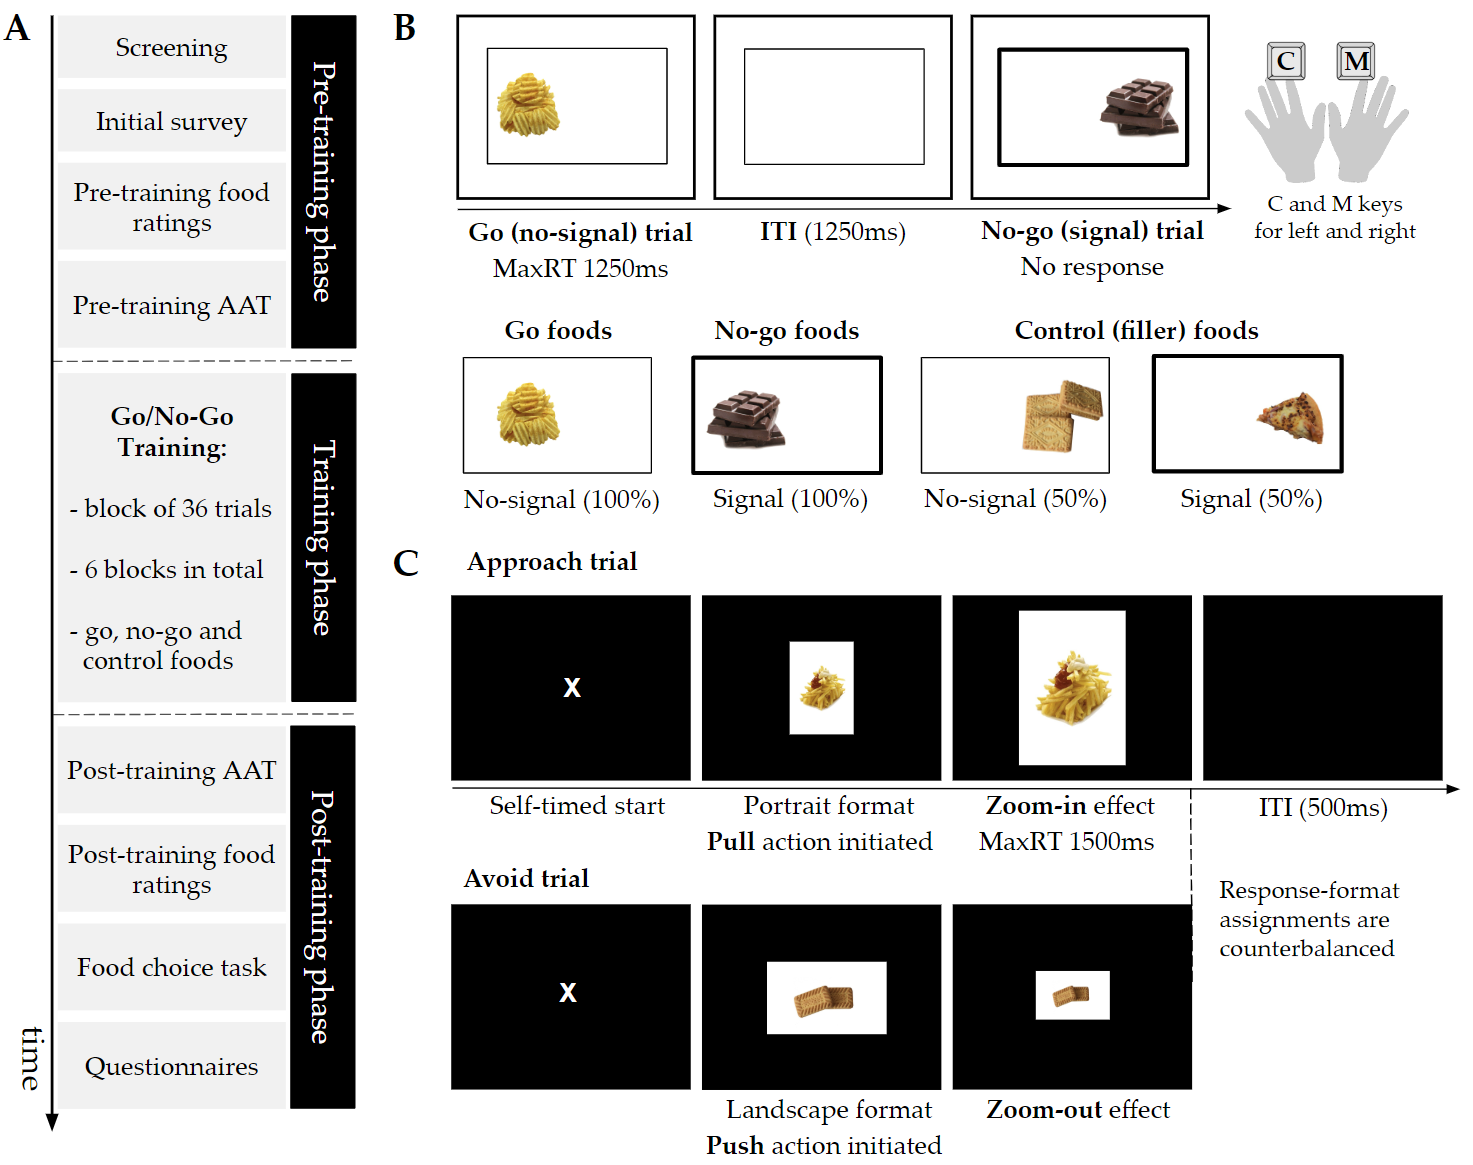
\includegraphics[width=\linewidth]{figures/Figure1.png}
\caption{\textbf{Schematic diagram of the study procedure, go/no-go training and approach-avoidance tasks.} \textbf{A.} After completing the screening and initial survey, participants rated all food stimuli (liking) and proceeded to perform the pre-training approach-avoidance task (AAT) blocks. In the training phase, participants completed six blocks of go/no-go training. The post-training AAT blocks were then presented and followed by food liking ratings. At the end of the study, participants completed a short food choice task and several questionnaires, in random order. \textbf{B.} The go/no-go training paradigm involved go (no-signal) and no-go (signal) trials that occurred with equal probability. On go trials, participants had to respond within 1250ms by pressing the "C" and "M" keys to indicate the picture location (left or right, respectively). On no-go trials, participants were instructed not to respond at all. The inter-trial interval (ITI) was 1250ms. Food categories were randomly assigned to three conditions. Go foods were only paired with no-signal trials and no-go foods were always associated with no-signal trials. Control, or filler, foods were presented in both signal and no-signal trials (50:50).}
\label{fig:procedure}
\end{figure}
\clearpage
\begin{figure}
    \ContinuedFloat
    \captionsetup{labelformat=empty}
    \caption{\textbf{C.} In the AAT, participants were asked to respond according to the format of the presented rectangle (portrait or landscape). Response-format assignments were approximately counterbalanced across participants. As an example, on approach trials a participant would have to pull the mouse towards them when the picture was in portrait format (approach trial) and push it away from them when the picture was in landscape format. Push and pull actions were paired with visual feedback, that is, zoom-out and zoom-in effects respectively. The maximum reaction time (maxRT) was 1500ms and the ITI was set to 500ms. Participants clicked on a central "X" to begin a trial (self-timed start).}
\end{figure}

\hypertarget{gng}{%
\subsection{Go/No-go training}\label{gng}}

\par

The Go/No-Go (GNG) training paradigm involved go and no-go responses to six pre-selected appetitive food categories. Food categories differed in terms of taste, so that three foods were savoury (i.e., pizza, crisps, chips) and three foods were sweet (i.e., biscuits, chocolate, cake)\footnote{All study materials are openly available at https://osf.io/wcf4r/}. Two food categories were randomly assigned to each training condition (go, no-go, filler foods) in the beginning of the experiment and food taste was counterbalanced so that each condition had one sweet and one savoury food. There were three training conditions according to the mapping of foods to signal (no-go) and no-signal (go) trials in the GNG. All go foods appeared in go (no-signal) trials and all no-go foods were presented in no-go (signal) trials (see Figure 1, panel C). Control, or filler, foods appeared on both go and no-go trials with equal probability (i.e., 50:50). Each food category had three exemplars which appeared twice in each block.

\par

All foods were presented on either the left or right hand side of the screen within a rectangle for 1250ms, which was the maximum reaction time (maxRT), as shown in Figure \ref{fig:procedure}, panel B. Participants were asked to respond to the location of the food as quickly and as accurately as possible by pressing the \enquote{C} and \enquote{M} buttons on the keyboard with their left and right index fingers, respectively. The central rectangle remained on the screen throughout the training, including the inter-trial-interval (ITI), which was 1250ms. On signal trials, the rectangle turned bold, indicating that participants should withhold their response. In line with the GNG training paradigm, this signal appeared on stimulus onset (i.e., no delay between stimulus and signal) and stayed on the screen until the end of the trial. A correct response on no-signal trials was registered when participants responded accurately to the location of the food within the maxRT window and a successful stop (i.e., correct signal trial) was considered when participants did not respond at all. Incorrect responses in no-signal trials refer to either to a wrong location judgement or a missed response. Left and right responses were counterbalanced across all manipulated variables for each type of trial. Training was split into 6 blocks of 36 trials (216 trials in total) and lasted approximately 10 minutes with inter-block breaks (15s). Task practice included 12 trials of go and no-go responses (50\%-50\%) and participants responded to the location of grey squares, instead of food pictures. For the practice trials, accuracy feedback was provided during the ITI.

\hypertarget{aat}{%
\subsection{Approach avoidance task}\label{aat}}

\par

The approach-avoidance task (AAT) was adapted from an existent paradigm (Rinck \& Becker, 2007; Wiers, Rinck, Dictus, \& Van Den Wildenberg, 2009), which involves \enquote{pull} (i.e., towards self) and \enquote{push} (i.e, away from self) movements of a joystick. Each type of motor response is paired with visual feedback so that when the joystick is pulled, the image gets bigger (zoom-in) and when it is pushed, the image gets smaller (zoom-out). This \enquote{zooming} effects acts as an exteroceptive cue of either an approach or avoidance response (Neumann \& Strack, 2000). This feature of the joystick AAT complements the proprioceptive properties of the task, where responses requiring arm flexion and extension correspond to approach and avoidance trials, respectively. This task also disambiguates approach and avoidance responses by using the \enquote{zooming} feature (Wiers et al., 2009), as previously explained. The evaluation-irrelevant feature of the paradigm was also incorporated and participants respond according to the format of the picture (portrait or landscape; e.g., Wiers et al., 2010).

\par

AAT responses involved \enquote{push} and \enquote{pull} movements of the computer mouse (adaptation of the joystick version). Food stimuli were presented in the centre of the screen and participants were instructed to pull the mouse towards them or push the mouse away from them according to whether the image was in portrait or landscape format (see Figure \ref{fig:procedure}, panel C). Response-format assignments were approximately counterbalanced across participants (45.4\% portrait-approach, 54.6\% landscape-approach). Instructions highlighted moving the mouse cursor until it reaches the end of the screen (top or bottom edge) for a correct response to be registered and making smooth whole-arm movements. Participants had 1500ms to respond after the stimulus appeared. Each trial started with a central \enquote{X} on the screen and participants had to click on it to begin (self-timed start). The ITI was 500 ms and there was no delay between the \enquote{X} click response and the stimulus onset. In order to account for the natural movement of the mouse, pixel tolerance was added to every mouse movement (\(\pm\) 1.25\% of display height), including movement initiation in the beginning of the trial. A response in the AAT was registered as correct only when participants completed the correct action (e.g., pull or push) within the maxRT window and also initiated a movement towards the correct direction. Even if the final response was correct, participants could have changed their movement after making an initial error (e.g., pull instead of push the mouse in an \enquote{avoid} trial) and therefore the direction of their initial movement was also taken into account. The complete RT for an AAT trial was defined as the time from the stimulus onset to the successful completion of a response.

\par

Each AAT block consisted of 72 trials and go, no-go and control foods appeared with equal probability for both \enquote{pull} (approach) and \enquote{push} (avoid) responses. There were 12 approach and 12 avoid trials for each training condition (e.g., no-go) and within those trials, there were six savoury and six sweet foods presented (i.e., three exemplars repeated twice). Three AAT blocks were performed before training (AAT\textsubscript{pre}) and three after training (AAT\textsubscript{post}). There was a number of constraints placed on the quasi-random order of the trials within an AAT block. There were no more than three images of the same food category being presented consecutively and no more than three trials with the same picture format in sequence. AAT practice consisted of 10 trials with grey rectangles instead of food stimuli and accuracy feedback. The screen background for the AAT was black and the task lasted approximately 15 minutes, including the inter-block 15s breaks, where participants received a reminder of the main instructions.

\hypertarget{food_ratings}{%
\subsection{Food liking ratings}\label{food_ratings}}

\par

Participants provided food liking ratings before and after training using a visual analogue scale (VAS). They rated all foods included in the GNG paradigm according to how much they liked the taste, ranging from 0 (\enquote{not at all}) to 100 (\enquote{very much}). Task instructions encouraged participants to imagine they were tasting the food in their mouth and then rate how much they liked the taste. The order of the presented foods was randomised and each block consisted of 18 trials. Participants completed a block before training (Liking\textsubscript{pre}) and a block after training (Liking\textsubscript{post}).

\hypertarget{food_choice}{%
\subsection{Food choice task}\label{food_choice}}

Impulsive food choices were assessed using a food choice task adapted from Veling et al. (2013a), which included all food categories from the GNG paradigm (two exemplars per category). The twelve foods were presented on a grid layout and participants had ten seconds to select three foods that they would like to consume the most at that specific time, by clicking on them with the computer mouse. Participants were asked to click on a \enquote{start} button to begin the trial and when a response was registered the selected food stimulus disappeared from the screen. It was assumed that this task element would prevent participants from deliberating on their choices and changing their initial responses, which would mean that \emph{impulsive} food choices were no longer measured. However, it should be noted that although participants were not informed about the hypothetical nature of their choices, it is highly probable that they would not consider their choices consequential (i.e., they would not think they would get a food item at the end of the study).

\hypertarget{questionnaires}{%
\subsection{Survey \& Questionnaires}\label{questionnaires}}

\par

Eligible participants were presented with an initial survey to record demographics and other variables for exploratory analyses. The survey consisted of height and weight measurements to calculate participant's body-mass-index (BMI; kg/m\(^{2}\)), the number of hours since their last meal (\enquote{less than 3 hours ago}, \enquote{3-5 hours ago}, \enquote{5-10 hours ago}, \enquote{more than 10 hours ago}) and hunger state at the the time of the study (VAS: 1=\enquote{Not at all} to 9=\enquote{Very}). Gender was also recorded with the options of male, female, transgender male, transgender female, gender variant/non-conforming, and an open ended text response for \enquote{other}.

\par

Several questionnaires were completed by the participants at the end of the study for exploratory analyses, as part of the undergraduate student projects of the GW4 Undergraduate Psychology Consortium 2017/2018. The Barratt Impulsivity Scale (BIS-15; Spinella, 2007) was introduced as a measure of impulsivity and the Stop Control Scale (SCS; De Boer, van Hooft, \& Bakker, 2011) was used to examine a distinctive element of general trait self-control, referred to as stop control. Other administered questionnaires included the Food Cravings Questionnaire - Trait - reduced (FCQ-T-r; Meule, Hermann, \& Kübler, 2014), Perceived Stress Scale (PSS; Cohen, Kamarck, \& Mermelstein, 1983) and the \enquote{food} and \enquote{money} subscales from the Delaying Gratification Inventory (DGI; Hoerger, Quirk, \& Weed, 2011). A correlation matrix of main questionnaire measures and sample characteristics can be found in Appendix \ref{appendix_cormatrix}.

\hypertarget{analyses}{%
\section{Analyses}\label{analyses}}

\hypertarget{measures-indices}{%
\subsection{Measures \& indices}\label{measures-indices}}

\par

The mean error rates in no-signal and signal trials as well as mean reaction time in no-signal trials (GoRT) from the GNG informed participant exclusions (see \textit{\nameref{data_exclusions}}). For the contingency learning manipulation check (H3, H4), measures included the proportion of successful stops from signal trials for no-go and control foods which were paired with a signal (control-nogo) and the mean GoRTs for each participant from correct go and control-go trials.

\par

Performance in the AAT\textsubscript{pre} and AAT\textsubscript{post} blocks was considered only for correct responses. Median RTs for \enquote{push} and \enquote{pull} responses from all training condition levels were calculated at a participant level\footnote{RTs were recorded continuously from movement initiation to response completion with samples every 33ms (two display refresh rates) to allow dynamic zoom-in/zoom-out effects based on participants' mouse movements. However, a bug was encountered with the version of the software and the temporal resolution at which coordinates and times were recorded was reduced. For this reason, linear interpolation was applied to increase the samples to 100 for every trial and obtain more precise RT measures. All details regarding this procedure and the software bug can be found in the analyses scripts.}. Medians were used instead of means as they are less sensitive to outliers in RT distributions and in line with previous literature (Wiers et al., 2009, 2010). The approach-avoid bias score for each condition was calculated as the difference between the median RTs for \enquote{push} and' pull' responses (MedianRT\textsubscript{push}- MedianRT\textsubscript{pull}). Bias scores were computed for both AAT\textsubscript{pre} and AAT\textsubscript{post} blocks. Positive scores indicate an approach bias towards the foods of interest and negative scores reflect avoidance for those foods. Change scores for approach-avoid biases from pre-to post-training (\(\Delta\)AAT bias score) were calculated for pre-registered analyses (H1). The proportion of correct responses for each AAT design cell informed participant exclusions.

\par

Participants were required to choose three foods out of twelve in the food choice task and selections could vary in their number for each training condition (go, no-go, control). Food choices were therefore normalised according to the total number of responses per participant (i.e., proportion). These calculated proportions, which were calculated for each participant were then compared across training conditions. for example, if a participant had chosen two go foods and one filler food, the probability (i.e., calculated proportion) of choosing a go food would be 0.667, the probability of choosing a filler food would be 0.333 and the probability of choosing a no-go food would be 0. Food rating VAS scores were averaged (mean) across the two foods per training condition (i.e., sweet and savoury foods for go, no-go and control conditions) and the three exemplars of each food. Changes in food liking were examined in terms of change scores (\(\Delta\)Food liking score) from pre-to-post training.

\hypertarget{data_exclusions}{%
\subsection{Data exclusions}\label{data_exclusions}}

\par

Participant-level data exclusions were conducted based on GNG training and AAT performance and participants who met any of the following criteria were excluded from all respective analyses. Participants who had a mean GoRT greater than three standard deviations from the group mean and percentage of correct responses in no-signal trials less than 85\% were excluded. Participants were also excluded if their percentage of errors in signal trials was greater than three standard deviations from the group mean and percentage of errors in either pre- or post- AAT blocks greater than 0.25. Additionally, participants who submitted a food rating of 50 (i.e., neutral) for 24 or more trials wither pre-or post-training would not be included as it was assumed that multiple such responses would indicate that participants used the default setting of the VAS and purposefully skipped the rating trials.

\hypertarget{prereg_analyses}{%
\subsection{Pre-registered analyses}\label{prereg_analyses}}

\par

Data pre-processing and analyses were conducted in RStudio (RStudio Team, 2016) and JASP (JASP Team, 2018). Pre-registered analyses are described under their pre-specified hypotheses, as presented in \textit{\nameref{hypotheses}}. For all Bayesian paired samples t-tests mentioned hereinafter, a prior with the \(\sqrt{2/2}\) scale parameter for the half-Cauchy distribution was used.

\noindent H1. The effect of training condition on the change in approach-avoid bias scores from pre-to post-training was examined using a Bayesian Repeated Measures ANOVA with the default prior settings (Rouder, Engelhardt, McCabe, \& Morey, 2016; Rouder, Morey, Speckman, \& Province, 2012) and participants treated as a nuisance term.

\begin{itemize}
\item[H1a.] $\Delta$AAT\textsubscript{nogo} <  $\Delta$AAT\textsubscript{control}  
\item[H1b.] $\Delta$AAT\textsubscript{go} >  $\Delta$AAT\textsubscript{control}
\end{itemize}

\noindent H2. Two Bayesian paired samples t-tests were conducted for the mean proportions of selected foods in the go and no-go training condition compared to the control.

\begin{itemize}
\item[H2a.] p(no-go) < p(control)
\item[H2b.] p(go) > p(control)
\end{itemize}

\noindent H3. The effect of training condition on the change in food liking from pre-to post-training was examined using a Bayesian Repeated Measures ANOVA, consistent with H1.

\begin{itemize}
\item[H3a.] $\Delta$Liking\textsubscript{nogo} < $\Delta$Liking\textsubscript{control}
\item[H3b.] $\Delta$Liking\textsubscript{go} > $\Delta$Liking\textsubscript{control}
\end{itemize}

\noindent H4. Contingency learning during go/no-go training was examined using Bayesian paired-samples t-tests for the percentage of successful inhibition trials and go reaction times.

\begin{itemize}
\item[H4a.] PCsignal\textsubscript{nogo} > PCsignal\textsubscript{control-nogo}
\item[H4b.] GoRT\textsubscript{go} < GoRT\textsubscript{control-go}
\end{itemize}

The evidential value of confirmatory findings was solely determined by the Bayesian tests outlined in this section, as previously explained (see \textit{\nameref{sampling}}. Frequentist tests were conducted in order to further the reproducibility of findings (e.g., potential use in meta-analyses). Paired samples t-tests were two-tailed, in line with the reported power analysis\footnote{Although Bonferroni corrections were pre-registered for paired sample t-tests for paired sample t-tests following Bayesian Repeated Measures ANOVAs, there were only two planned contrasts for each ANOVA and reflected distinct hypotheses about the data. Therefore, such corrections were not applied for the reported p-values.} Assumptions for repeated measures ANOVAs (H1 and H3) were checked in line with the pre-registered analysis plan and no violations were observed. Contingency plans were not considered in case the normality assumption was violated for paired t-tests (Shapiro Wilk test: \emph{p} \(\leq\) .005), but appropriate exploratory analyses were conducted and reported in the \textit{\nameref{robust}} section\footnote{For other analyses reported in the \textit{\nameref{exploratory_findings}} section, p-values from Wilcoxon signed-rank tests are reported as \textit{p\textsubscript{W}} in a supplementary manner.}. A minor deviation from the pre-registered frequentist analyses was that paired sample t-tests for H1a and H1b were conducted irrespective of the Repeated Measures ANOVA results (H1).

\hypertarget{results}{%
\section{Results}\label{results}}

\hypertarget{sample-characteristics}{%
\subsection{Sample characteristics}\label{sample-characteristics}}

The final sample for pre-registered analyses consisted of 163 participants (80.98\% female). Detailed participant-level exclusions are presented in Figure A1. Participants had on average a healthy BMI (\emph{M} = 22.88, \emph{SD} = 2.98, range = 18.54 - 32.36) and their mean age was 22.39 (\emph{SD} = 9.04, range = 18-59). 108 participants (66.26\%) reported that they had their last meal 3-5 hours before the study and hunger levels at the beginning of the study were not particularly high (\emph{M} = 5.70, \emph{SD} = 2.22). However, 24 participants (14.72\%) did not adhere to the instruction not to eat three hours before the study, as they reported having their last meal \enquote{less than 3 hours ago}.

\hypertarget{confirmatory_findings}{%
\subsection{Confirmatory findings}\label{confirmatory_findings}}

\hypertarget{training_outcomes}{%
\subsubsection{Training outcomes}\label{training_outcomes}}

\par

There was \emph{strong} evidence for the absence of a general effect of go/no-go training condition on the change in approach-avoidance bias scores {[}\emph{BF}\(_{01}\) = 16.06; \emph{F}(2, 324) = 1.01, \emph{p} = 0.365{]}. Results for paired comparisons are shown in Table 1. There was \emph{moderate} evidence that the change in bias scores for no-go foods (\(\Delta\)AAT\textsubscript{nogo}; \emph{M} = -3.31, \emph{SD} = 62.91) was not reduced compared to the change for filler foods (\(\Delta\)AAT\textsubscript{control}; \emph{M} = -1.81, \emph{SD} = 59.55). Similar to H1a, there was \emph{strong} evidence for the null compared to the alternative for H1b. The change in bias scores for go foods (\(\Delta\)AAT\textsubscript{go}; \emph{M} = -10.47, \emph{SD} = 59.57) was not greater than the change for filler foods. Approach-avoidance bias scores pre- and post- training across training conditions can be visualised using rainclouds in Figure \ref{fig:raincloud_bias}. The raincloud plots have been created using existing code and guidelines (Allen, Poggiali, Whitaker, Marshall, \& Kievit, 2019, 2018).

\par

The effect of training on impulsive food choices was examined for no-go and go foods compared to control, as stated in H2a and H2b respectively. There was \emph{extreme} evidence that the probability of choosing a no-go food (\emph{M} = 0.21, \emph{SD} = 0.27) was reduced compared to the probability of choosing a filler food (\emph{M} = 0.36; \emph{SD} = 0.31) after training\footnote{There was a missing value for this analysis as one participant did not complete the food choice task.} (see Table 1). In contrast, there was only \emph{anecdotal} evidence that probability of choosing a go food (\emph{M} = 0.44; \emph{SD} = 0.33) was not greater than the probability of choosing a filler food after training.

\begin{figure} [!htb]
\centering
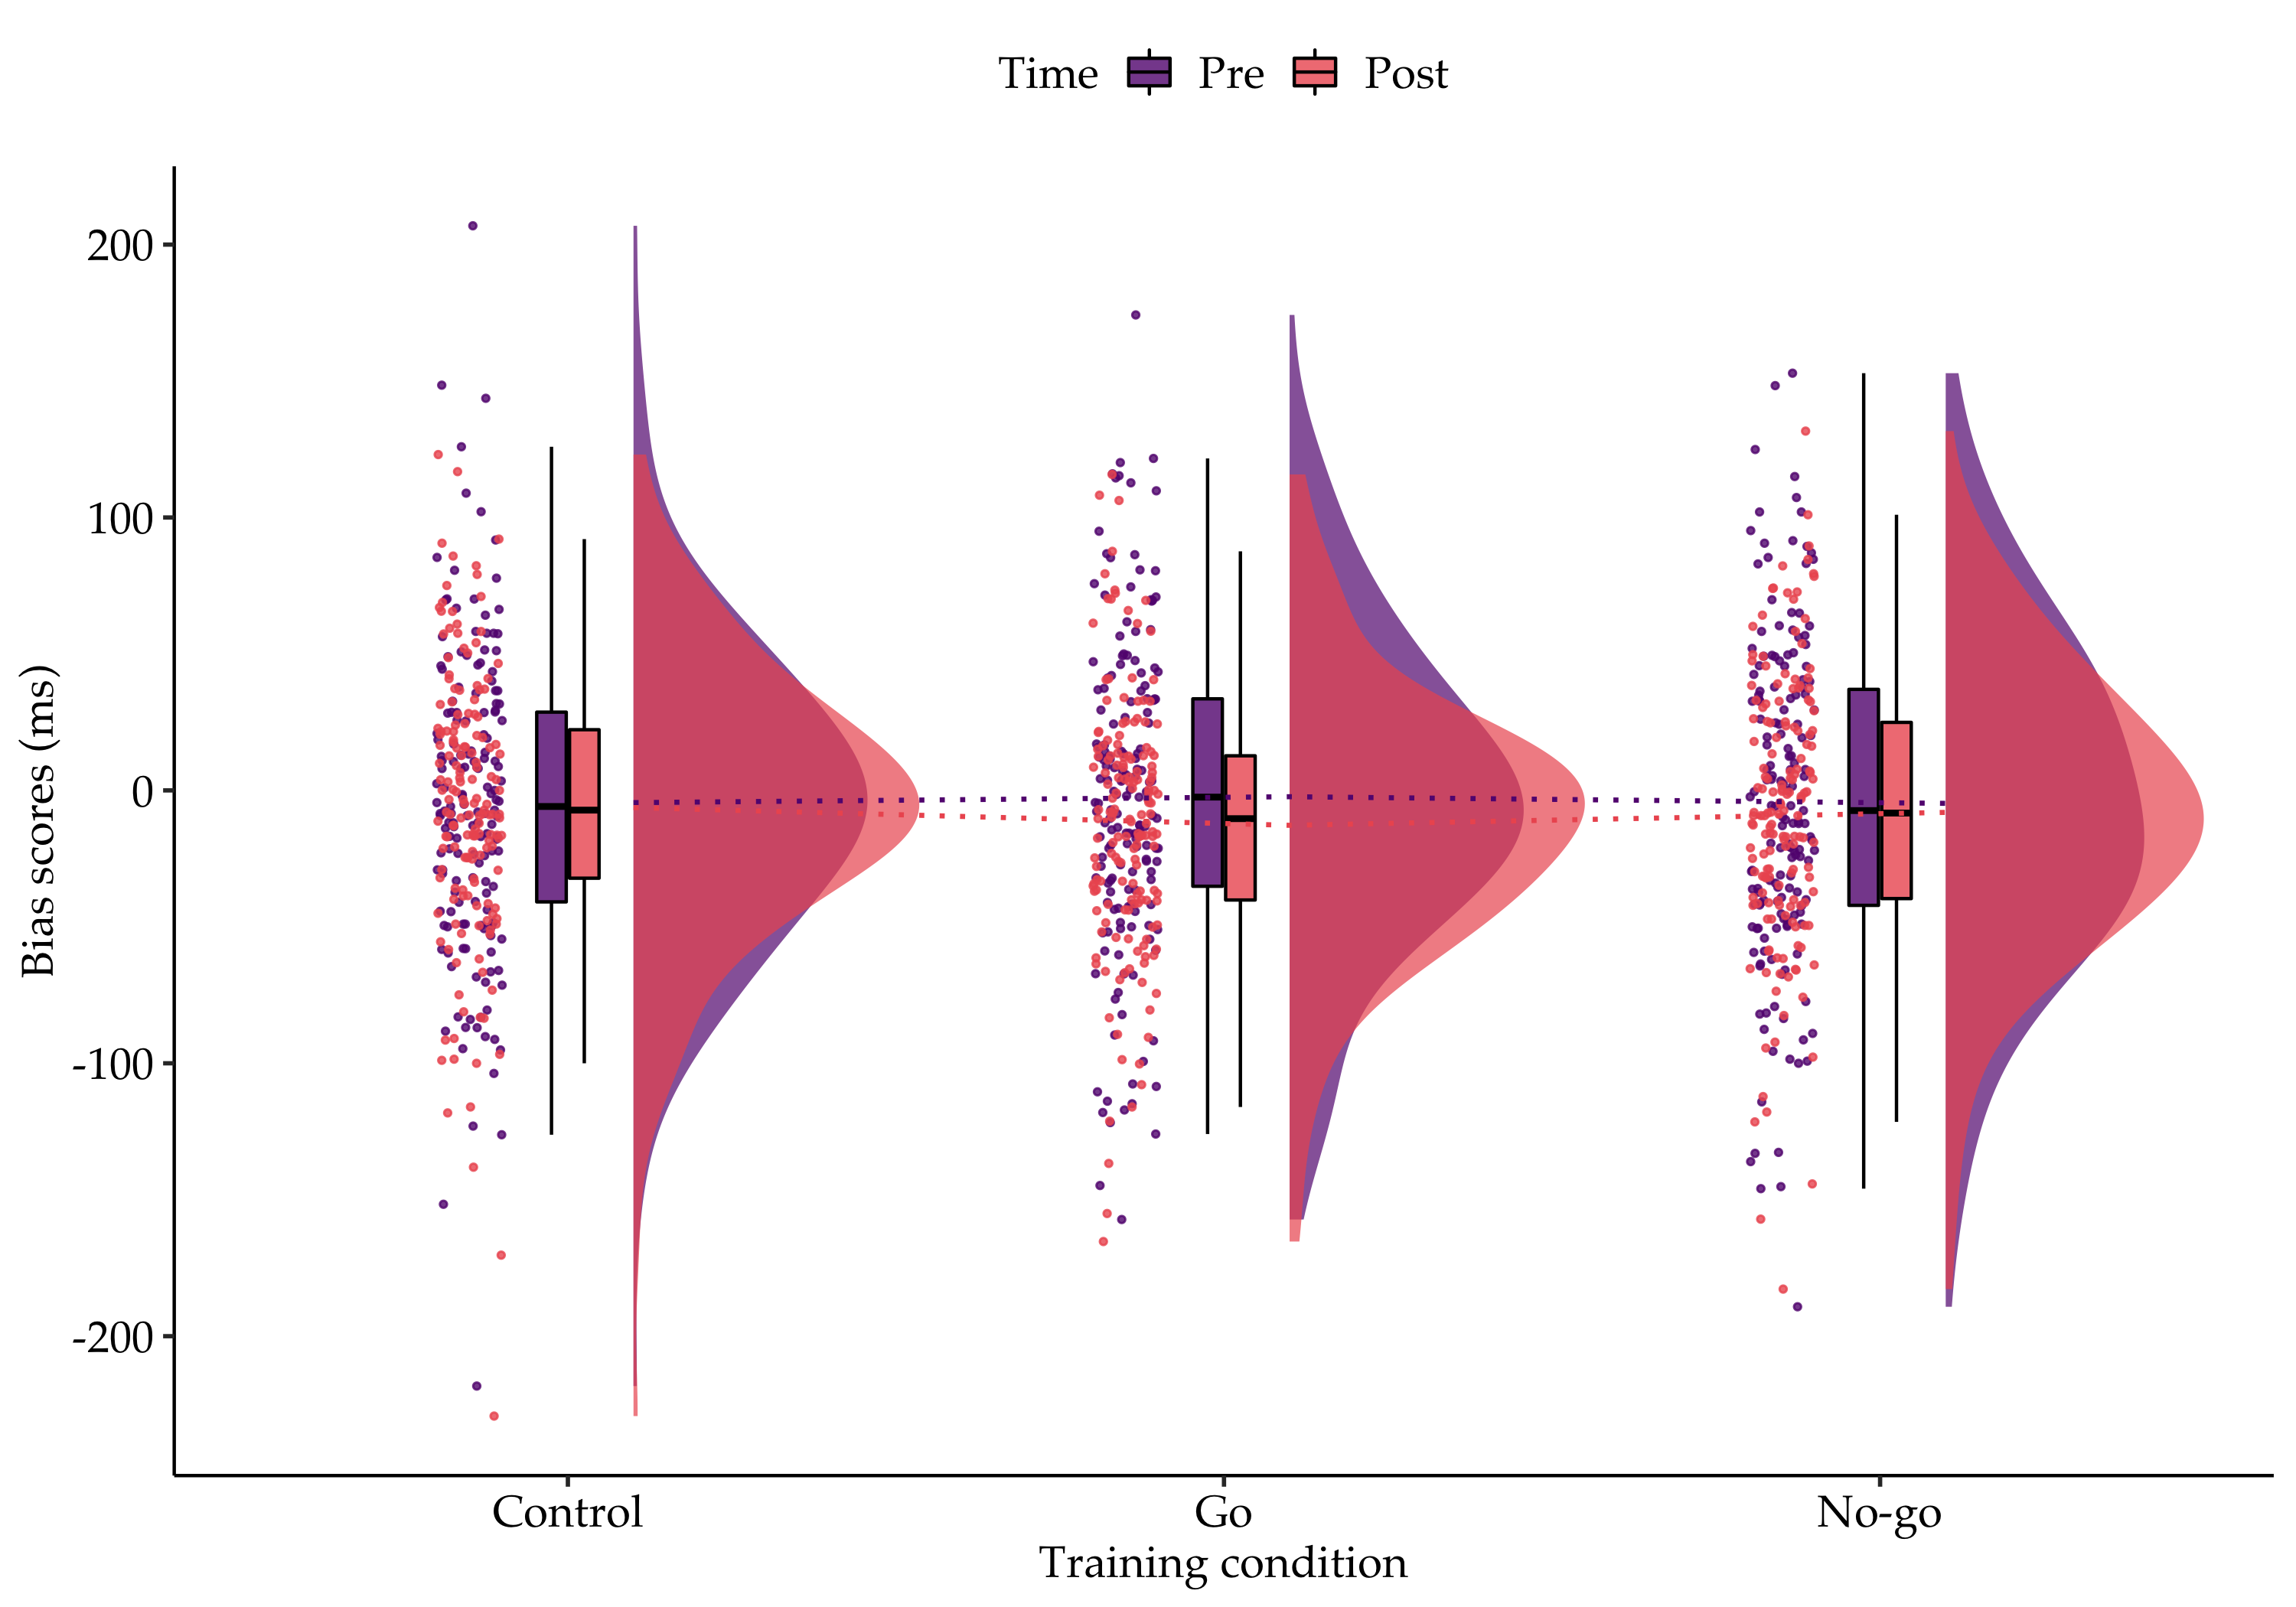
\includegraphics[width=\linewidth]{figures/Figure2.png}
\captionof{figure}{\textbf{Raincloud plot of the approach-avoidance bias scores pre- and post- training across training conditions.} There were no differences between the sample mean changes in approach-avoidance bias scores for no-go and go foods compared to control (filler) foods, as shown by the dashed lines. At a closer inspection, individual bias scores do not seem to be clustered around the positive end of the distribution as it would be expected for for appetitive unhealthy foods, but actually show less dispersion around zero. Exploratory analyses confirmed that baseline bias scores did not statistically deviate from zero (see \textit{\nameref{baseline_bias}}). \textit{Note.} The `split-half violin' elements in the plot show smoothed distributions.} 
\label{fig:raincloud_bias}
\end{figure}

\begin{table}[!htb]
    \centering
    \caption{Results for all pre-registered hypotheses and respective statistical tests}
    \label{tab:preregistered}
    {
        \begin{tabular}{lrrrrrrrr}
            \toprule
         &   &  &  &  &  & \multicolumn{2}{c}{95\% CI for \textit{d}} & \\
            \cline{7-8}
             & \textit{BF}\textsubscript{10} & \textit{t} & \textit{df} & \textit{p} & \textit{d} & Lower & Upper  & Evidence interpretation \\
            \cmidrule(r){1-9}
            H1a & 0.107 & -0.25 & 162 & 0.805 & -0.02 & -0.17 & 0.13 & \textit{Moderate} evidence for H\textsubscript{0} \\
            H1b & 0.039 & -1.35 & 162 & 0.179 & -0.11 & -0.26 & 0.05 & \textit{Strong} evidence for H\textsubscript{0} \\
            H2a & 247.782 & -3.93 & 161 & < .001 & -0.31 & -0.47 & -0.15 & \textit{Extreme} evidence for H\textsubscript{1} \\
            H2b & 0.849 & 1.82 & 161 & 0.070 & 0.14 & -0.01 & 0.30 & \textit{Anecdotal} evidence for H\textsubscript{0} \\
            H3a & 2.648 & -2.38 & 162 & 0.019 & -0.19 & -0.34 & -0.03 & \textit{Anecdotal} evidence for H\textsubscript{1} \\
            H3b & 0.067 & -0.37 & 162 & 0.715 & -0.03 & -0.18 & 0.13 & \textit{Strong} evidence for H\textsubscript{0} \\
            H4a & 140.254 & 3.77 & 162 & < .001 & 0.30 & 0.14 & 0.45 & \textit{Extreme} evidence for H\textsubscript{1} \\
            H4b & 3973.214 & -4.66 & 162 & < .001 & -0.37 & -0.52 & -0.21 & \textit{Extreme} evidence for H\textsubscript{1} \\
            \bottomrule
        \end{tabular}
    }
        \begin{tablenotes}[para]
\footnotesize{\textit{Note.} Evidence is interpreted for the alternative hypothesis (H\textsubscript{1}) compared to the null (H\textsubscript{0}) and vice versa. All Bayesian paired samples t-tests were directional, as indicated in the \textit{\nameref{prereg_analyses}} section and frequentist equivalents were non-directional (two-tailed). The effect size is represented by Cohen's \textit{d}.}
\end{tablenotes}
\end{table}

\hypertarget{manipulation_checks}{%
\subsubsection{Manipulation checks for training}\label{manipulation_checks}}

\par

As a first manipulation check for training outcomes, it was investigated whether GNG changed the evaluations of foods associated with signal and no-signal trials compared to the evaluations of filler foods which were paired with either type of trial with equal probability (control). There was only \emph{anecdotal} evidence for the absence of a general effect of training condition on the changes in liking from pre- to post- training {[}H3; \emph{BF}\textsubscript{01} = 2.89; \emph{F}(2, 324) = 2.90, \emph{p} = 0.057{]}. The change in liking scores from pre-to post-training for nogo foods (\(\Delta\)Liking\textsubscript{nogo}; \emph{M} = -4.16; \emph{SD} = 9.51) was only slightly reduced compared to change in liking for filler foods (\(\Delta\)Liking\textsubscript{control}; \emph{M} = -2.61, \emph{SD} = 8.77), and there was only \emph{anecdotal} evidence for this effect (H3a; see Table 1). The change in liking scores from pre-to post-training for go foods (\(\Delta\) Liking\textsubscript{go}; \emph{M} = -2.87, \emph{SD} = 10.15), however, was not greater than the change for filler foods as originally expected. Instead, there was \emph{strong} evidence for the null hypothesis compared to the alternative (H3b).

\begin{figure} [!htb]
\centering
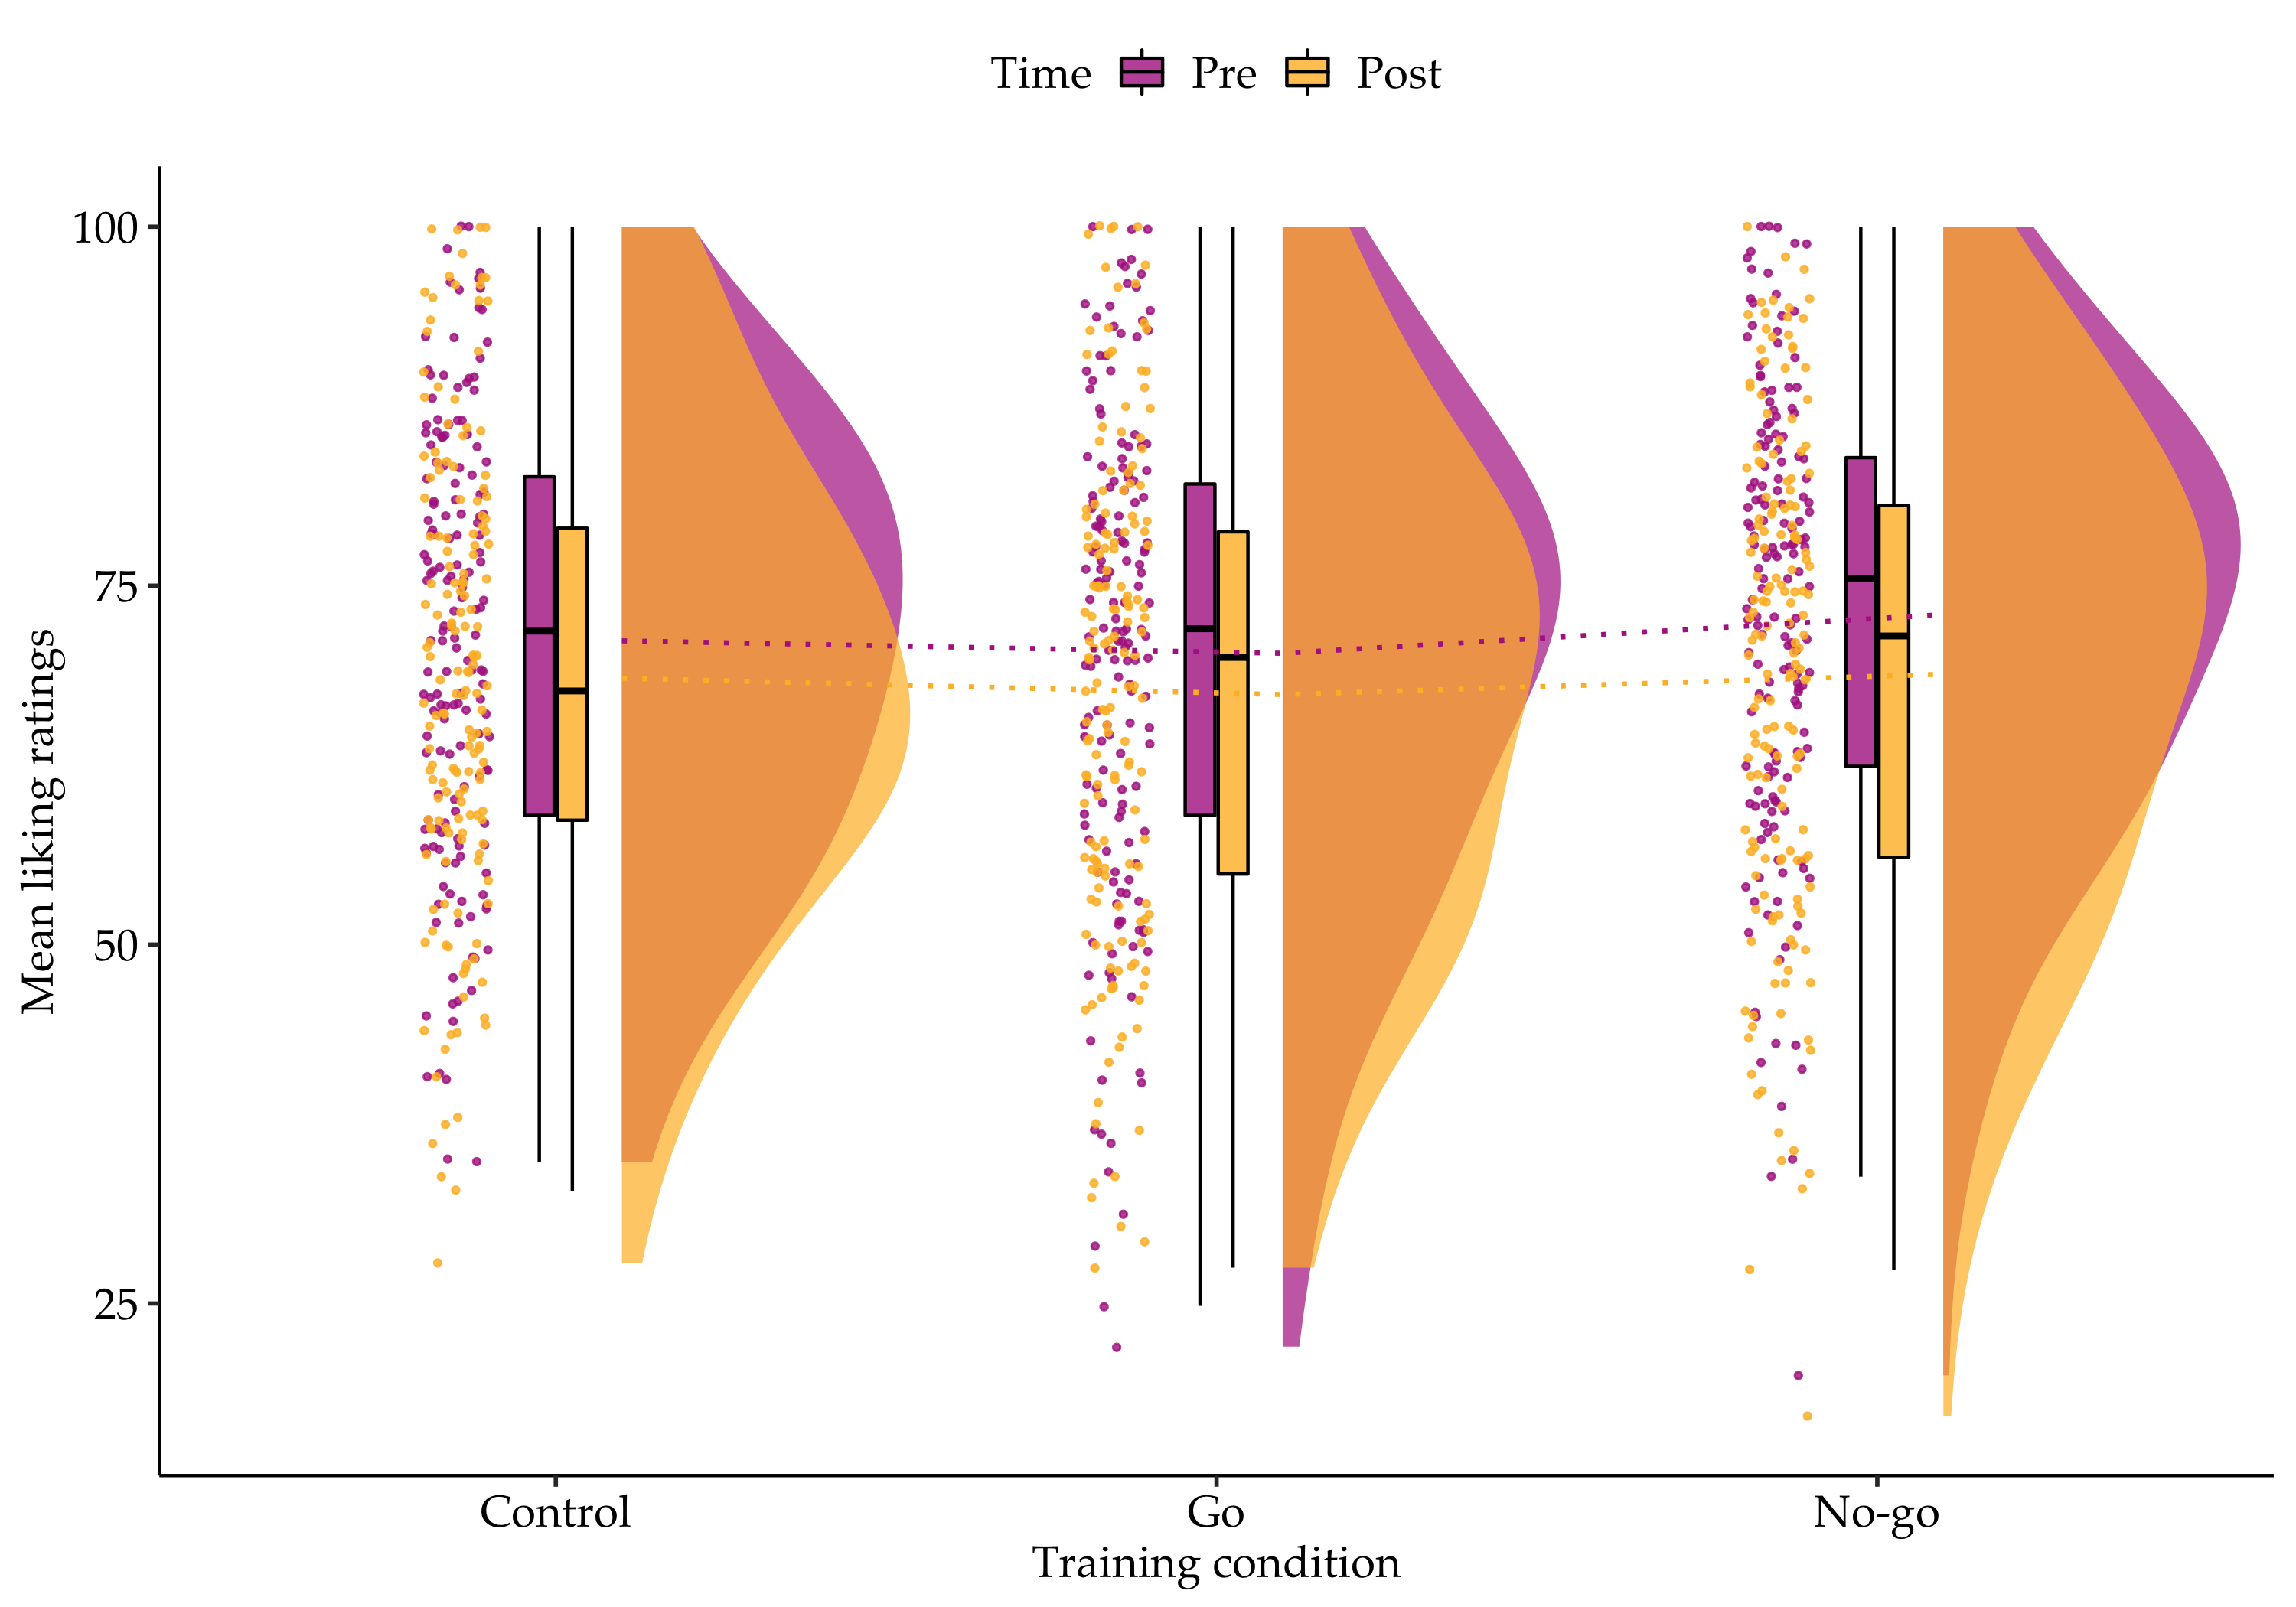
\includegraphics[width=\linewidth]{figures/Figure3.png}
\captionof{figure}{\textbf{Raincloud plot of the mean liking ratings pre- and post- training across training conditions.} This visualisation of the mean liking ratings from all participants revealed that the distributions are more skewed than expected, towards the least liked range of the visual analogue scale (VAS). Taste (liking) ratings were registered on a VAS ranging from 0 to 100 (i.e., 50=neutral). Although there appears to be a small difference between the change in liking for no-go foods compared to the control, the trends presented in this plot were inspected further to establish whether observed effects were robust (see \textit{\nameref{robust}}). Also, there appears to be a general trend of devaluation across training conditions and this was statistically supported (see \textit{\nameref{devaluation_trends}}). \textit{Note.} The `split-half violin' elements in the plot show smoothed and trimmed distributions.} 
\label{fig:raincloud_liking}
\end{figure}

\par

In order to validate whether the implemented go/no-go training paradigm led to stimulus-response associations (i.e., contingency learning), it was tested whether the percentage of correct responses for no-go foods (i.e., successful inhibitions) would be greater compared to the percentage of correct responses for filler foods associated with signal trials (H4a). There was \emph{extreme} evidence that participants had on average more successful inhibitions for no-go foods (PCsignal\textsubscript{nogo}; \emph{M} = 0.97, \emph{SD} = 0.03) than filler foods
(PCsignal\textsubscript{control-nogo}; \emph{M} = 0.96, \emph{SD} = 0.04). For H4b, it was examined whether mean reaction times would be reduced for go foods (GoRT\textsubscript{go}; \emph{M} = 507.00, \emph{SD} = 70.48) compared to filler foods associated with no-signal trials (GoRT\textsubscript{control-go}; \emph{M} = 515.00, \emph{SD} = 75.51) and there was \emph{extreme} evidence for such an effect. Therefore, contingency learning was observed in the employed GNG paradigm for both reaction time and accuracy outcomes.

\begin{figure} [!htb]
\centering
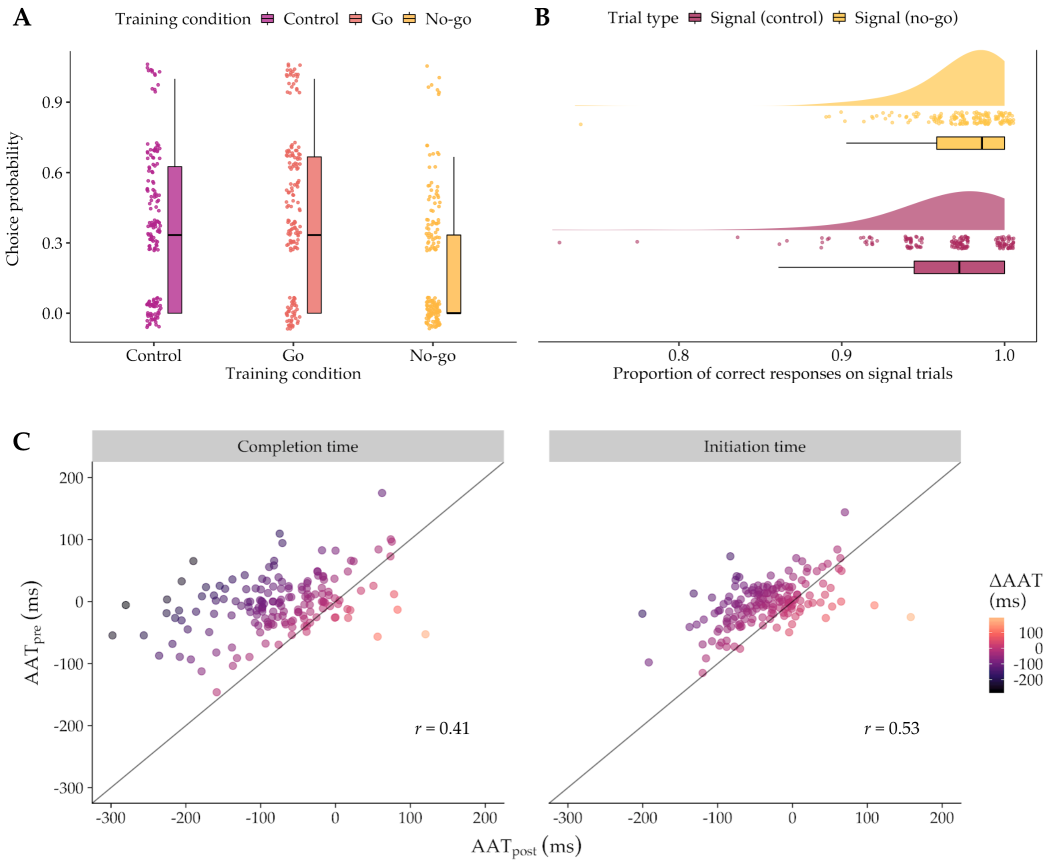
\includegraphics[width=\linewidth]{figures/Figure4.png}
\captionof{figure}{\textbf{Plots for food choice outcomes, accuracy-based contingency learning in training and test-retest reliability of approach-avoidance bias scores.} \textbf{A.} The boxplots with corresponding jittered individual data points clearly show that the probability of choosing a no-go food after training is reduced compared to the probability of choosing control food [H2a]. Contrary to initial predictions, the average choice probability was not greater for go foods relative to the control [H2b]. \textbf{B.} The proportion of correct responses on signal trials (PC\textsubscript{signal}) was relatively greater for no-go foods compared to control foods. The PC\textsubscript{signal} distribution for control foods was heavily skewed and this observation warranted a robustness check for effect estimates, as presented in the \textit{\nameref{robust}} section.} 
\label{fig:multipanel}
\end{figure} 
\clearpage
\begin{figure}
    \ContinuedFloat
    \captionsetup{labelformat=empty}
    \caption{\textbf{C.} For the pre-registered analysis of training outcomes on automatic action tendencies [H1], approach-avoidance bias scores ($\Delta$AAT) were calculated based on median reaction times for correct pull and push responses from pre-to post-training (AAT\textsubscript{post} - AAT\textsubscript{pre}). These reaction times refer to the time participants took to complete an action (i.e., completion time). TThe test-retest reliability for the calculated scores is poor (Pearson’s *r* coefficient = 0.41; see \textit{\nameref{reliability}} for detailed results). When bias scores are computed using the time when participants initiated a movement since stimulus onset on a correct trial (i..e, initiation times), the test-retest reliability was slightly improved (r = 0.53) and less dispersion was observed for $\Delta$AAT across participants. \textit{Note.} The `split-half violin' elements in the plot show smoothed and trimmed distributions. Individual data points have been jittered  to some degree due to overfitting, as it can be seen for the cluster of data points in panel B for very high proportions of correct responses on signal trials.}
\end{figure}

\hypertarget{exploratory-findings}{%
\subsection{Exploratory findings}\label{exploratory-findings}}

\hypertarget{baseline_bias}{%
\subsubsection{Baseline approach bias scores}\label{baseline_bias}}

Performance in the AAT was inspected further to check if approach bias for foods was present in the final sample and whether error rates differed across conditions. Although the sample means for AAT\textsubscript{pre} bias scores are negative for go foods (\emph{M} = -2.32, \emph{SD} = 58.14), no-go foods (\emph{M} = -4.75, \emph{SD} = 60.58) and filler foods (\emph{M} = -4.48, \emph{SD} = 52.25), individual data points (see Figure \ref{fig:raincloud_bias} show less dispersion close to zero, suggesting that neither approach or avoidance bias was captured by the AAT. In line with previous literature (see Table 1 in Becker et al., 2015), this hypothesis was directly tested by examining whether baseline bias scores statistically deviated from zero using Bayesian one sample t-tests with the default prior settings for the two-sided alternative hypothesis that the population mean was larger than the test value. Equivalent frequentist tests were also conducted. Overall, conclusive evidence for the absence of baseline approach/avoidance bias was obtained for any of the foods which were randomly assigned to training conditions (see Table \ref{tab:baseline}).

\par

As baseline bias scores calculated from completion times may be \enquote{contaminated} by motor demands in this version of the AAT that requires computer mouse movements and arm flexion/extension, the possibility that motor initiation times may be more sensitive to capturing automatic action tendencies was considered. Movement initiation was registered when participants had moved their mouse cursor since starting a trial (i.e., stimulus onset), including the pixel tolerance for natural movements of the mouse (see \textit{\nameref{aat}}). Therefore, tests were also conducted for baseline bias scores calculated using median initiation times, instead of median completion times. Consistent with the results presented above, there was strong evidence that baseline bias scores did not deviate from zero across training conditions (see Table \ref{tab:baseline}).

\begin{table}[h] 
    \centering
    \caption{Results of Bayesian and frequentist one sample t-tests for baseline approach-avoidance bias scores}
    \label{tab:baseline}
    {
        \begin{tabular}{lrrrrrr}
            \toprule
             &  &  &  & & \multicolumn{2}{c}{95\% CI for \textit{d}} \\
            \cline{6-7}
             & \textit{BF}\textsubscript{01}  & \textit{t}(162) & \textit{p} & \textit{d} & Lower & Upper \\
            \cmidrule(r){1-7}
            Completion time: AAT\textsubscript{pre} for go foods  & 10.08 & -0.51& 0.611 & -0.04 & -0.19 & 0.11  \\
            Completion time: AAT\textsubscript{pre} for no-go foods  & 7.01 & -1.00 & 0.318 & -0.08 & -0.23 & 0.08 \\
            Completion time: AAT\textsubscript{pre} for control foods  & 7.02 & -1.00 & 0.319 & -0.08 & -0.23 & 0.08 \\
            Initiation time: AAT\textsubscript{pre} for go foods  & 10.73 & -0.36 & 0.718 & -0.03 & -0.18 & 0.13  \\
            Initiation time: AAT\textsubscript{pre} for no-go foods  & 10.18 & -0.49 & 0.626 & -0.04 & -0.19 & 0.12 \\
            Initiation time: AAT\textsubscript{pre} for control foods  & 10.46 & -0.43 & 0.669 & -0.03 & -0.19 & 0.12 \\
            \bottomrule
        \end{tabular}
    }
    \begin{tablenotes}[para]
\footnotesize{\textit{Note.} AAT\textsubscript{pre}: Pre-training approach avoidance task bias scores}
\end{tablenotes}
\end{table}

\hypertarget{subgroup}{%
\subsubsection{Sub-group analysis}\label{subgroup}}

In an effort to show that training did not have an effect on AAT outcomes was not due to the absence of baseline approach bias for unhealthy foods, a sub-group analysis for participants with positive baseline bias scores (N=72) was conducted. There was \emph{very strong} evidence for the absence of a main effect of go/no-go training condition on the change in approach-avoidance bias scores {[}\emph{BF}\(_{01}\) = 43.99; \emph{F}(2, 142) = 0.01, \emph{p} = 0.987{]}. For this sub-group food-choice outcomes were consistent with the confirmatory findings reported in \textit{\nameref{training_outcomes}}. There was \emph{strong} evidence that the probability of choosing a no-go food (\emph{M} = 0.20, \emph{SD} = 0.27) was reduced relative to the probability of choosing a control food (\emph{M} = 0.37, \emph{SD} = 0.33) {[}\textit{BF}\textsubscript{10} = 13.97; \emph{t}(70){]} = -2.96, \emph{p} = 0.004, \textit{\textsubscript{W}} = 0.004, \emph{d} = -0.35, 95\% CI for \emph{d} = -0.59, -0.11{]}. There was \emph{moderate} evidence for the absence of a general effect of training condition on the change in liking scores from pre-to post-training {[}\emph{BF}\textsubscript{01} = 8.91; \emph{F}(2, 142) = 0.94, \emph{p} = 0.392{]}. With regards to the contingency learning manipulation check, there was\emph{very strong} evidence for a greater proportion of correct responses in signal trials with no-go foods compared to control foods {[}\emph{BF}\textsubscript{10} = 37.80; \emph{t}(71) = 3.33, \emph{p} = 0.001,\textit{\textsubscript{W}} \textless{} .001, \emph{d} = 0.39, 95\% CI for \emph{d} = 0.15, 0.63{]}. However, there was only \emph{anecdotal} evidence that GoRTs were faster for go foods compared to control foods {[}\emph{BF}\textsubscript{10} = 3.52; \emph{t}(71)) = -2.38, \emph{p} = 0.020, \emph{d} = -0.28, 95\% CI for \emph{d} = -0.52, -0.04{]}.

\hypertarget{accuracy_aat}{%
\subsubsection{Accuracy in the approach-avoidance task}\label{accuracy_aat}}

\par

Although reaction times are the primary measure of interest for studies that utilise the AAT so that bias scores can be calculated, an exploratory examination of error rates is also reported. At baseline, average error rates were not increased for trials where participants were required to avoid an appetitive food and complete a push action (\emph{M} = 0.136; \emph{SD} = 0.070) relative to trials where an approach (pull) action was completed (\emph{M} = 0.143; \emph{SD} = 0.066) {[}\textit{BF}\textsubscript{01} = 26.49; \textit{t}(162) = 1.42, \textit{p}= 0.159, \textit{d} = 0.11, 95\% CI for \textit{d} = -0.04, 0.26{]}. However, after training participants had on average more errors in approach trials (\emph{M} = .124, \emph{SD} = .074) compared to avoid trials (\emph{M} = 0.105, \emph{SD} = 0.062) {[}\textit{BF}\textsubscript{10} = 90.98, \textit{t}(162) = 3.64, \textit{p} \textless{} .001, \textit{p\textsubscript{W}} \textless{} .001, \textit{d} = 0.29, 95\% CI for \textit{d} = 0.13, 0.44{]}. It is possible that training had a \enquote{hidden} effect on accuracy, for example it was more difficult to approach no-go foods compared to go and/or control foods due to a learned association between response inhibition and these food stimuli. Difference scores were calculated from the mean error rates post-training (pull - push) to check whether this increase in error rates was general or specific to training conditions. There was very strong evidence for the absence of a general effect of training condition on differences in mean error rates between approach and avoid trials {[}H3; \emph{BF}\textsubscript{01} = 37.16; \emph{F}(2, 324) = 0.17, \emph{p} = 0.844{]}. RT differences between approach and avoid trials were inspected and there was \emph{strong} evidence for slower RTs on pull compared to push actions after training {[}\emph{BF}\textsubscript{10} = 11.32; \emph{t}(162) = 2.95, \emph{p} = 0.004, \textit{p\textsubscript{W}} = 0.002, \emph{d} = 0.23, 95\% CI for \emph{d} = 0.08, 0.39{]}. Together these results may indicate fatigue effects associated with bio-mechanical costs (e.g., arm flexion muscle group activation).

\hypertarget{reliability}{%
\subsubsection{Reliability of calculated bias scores}\label{reliability}}

Given the absence of evidence for baseline approach-avoidance bias scores deviating from zero and the variability in the distribution of score from negative to positive bias (see Figure 2), the test-retest reliability of the task measures was assessed. Considering that the the interval between pre- and post-training AAT blocks was very short and there could be added variability (i.e.~noise) due to the GNG intervention, a test-retest reliability (or stability) coefficient \emph{r} within the range of 0.6-0.7 would be considered adequate in this context. Test-retest reliability was assessed via correlation pairs for AAT bias scores at baseline (AAT\textsubscript{pre}) and after training (AAT\textsubscript{post}), as shown in Figure \ref{multipanel} (panel C). Consistent with the previous analyses of baseline bias scores (see \textit{\nameref{baseline_bias}}), test-retest reliability was examined for both completion time and initiation time AAT bias scores. Bayesian correlation pairs with the default prior (stretched beta with \(\gamma\)=1; Wagenmakers, Verhagen, and Ly (2016)) were used for these analyses. As expected, there was \emph{extreme} evidence for a positive linear relationship between completion time bias scores for pre- and post- training blocks, but the correlation coefficient (Pearson's rho) was only 0.41, indicating that there test-retest reliability of AAT bias scores based on completion times was poor {[}log(\textit{BF}\textsubscript{10}) = 12.95, \emph{p} \textless{} .001, 95\% CI for \emph{r} = 0.30, 1{]}. As discussed earlier, bias scores based on median completion times could be affected by noise in motor times and scores based on median initiation times would better reflect underlying cognitive processes, such as \emph{automatic} action tendencies. The test-retest reliability for bias scores based on initiation times however was only slightly better compared to completion time bias scores with a stability coefficient of 0.53 {[}log(\textit{BF}\textsubscript{10}) = 24.34, \emph{p} \textless{} .001, 95\% CI for \emph{r} = 0.43, 1{]}.

\hypertarget{devaluation_trends}{%
\subsubsection{Devaluation trends across training conditions}\label{devaluation_trends}}

As explained in Figure \ref{fig:raincloud_liking}, there was a general trend of devaluation in the data for all training conditions from pre- to post-training. These observed differencesw were tested directly and there was conclusive evidence that within each training condition cell, there is a negative change in mean liking ratings from pre- to post-training, as observed in Figure \ref{fig:raincloud_liking}. The control (filler) foods should be unaffected in terms of affective evaluation changes, but participants rated filler foods more negatively after training (\emph{M} = 68.55, \emph{SD} = 15.81) relative to baseline (\emph{M} = 71.16, \emph{SD} = 14.80) {[}\emph{BF}\textsubscript{10} = 156.54, \emph{t}(162) = 3.80, \emph{p} \textless{} .001, \textit{p\textsubscript{W}} = 0.001, \emph{d} = 0.30, 95\% CI for \emph{d} = 0.14, 0.45{]}. Contrary to predictions about the increase in positive evaluations for go foods (relative to control), within that condition cell the evaluations of go foods were less positive after training (\emph{M} = 67.42, \emph{SD} = 16.85) compared to before (\emph{M} = 70.29, \emph{SD} = 16.80) {[}\emph{BF}\textsubscript{10} = 84.52, \emph{t}(162) = 3.62, \emph{p} \textless{} .001, \textit{p\textsubscript{W}} \textless{} .001, \emph{d} = 0.28, 95\% CI for \emph{d} = 0.13, 0.44{]}. The effect was greater for no-go foods, but this is the only data trend that was theoretically consistent with effects of training. Participants provided less positive ratings for no-go foods after training (\emph{M} = 68.83, \emph{SD} = 16.81) compared to before (\emph{M} = 72.99, \emph{SD} = 15.38) {[}\emph{BF}\textsubscript{10} = 211398.68, \emph{t}(162) = 5.58, \emph{p} \textless{} .001, \textit{p\textsubscript{W}} \textless{} .001, \emph{d} = 0.44, 95\% CI for \emph{d} = 0.28, 0.60{]}.

\hypertarget{glm}{%
\subsubsection{General linear model of food choice data}\label{glm}}

\par

As shown in Figure 4 and as expected for counts data, food choice probabilities were not normally distributed and the inferences based on paired t-tests would need to be validated further. Choice count data from the impulsive food choice task were modelled using a general linear model (GLM) in R (R Core Team, 2017). The error term of the model was specified with a Poisson distribution and the link function log-transformed the linear predictor within the model (i.e., logarithms of fitted means). The only predictor in this model was the training condition (i.e.., go, no-go, or filler foods), with filler, or control, foods set as the reference point (i.e., intercept). Diagnostic plots showed mild violations of the assumptions of homoskedasticity and normality of residuals and thus robust standard errors for the parameter estimates were computed (Cameron \& Trivedi, 2009). An overdispersion test (Cameron \& Trivedi, 2005; Kleiber \& Zeileis, 2008) showed that true dispersion was not greater than 1 and the goodness-of-fit chi-squared test was not statistically significant, indicating that the model had a good fit (Residual variance = 436.15, df = 486, \emph{p} = 0.949). The GLM results are consistent with the pre-registered statistical test results (see Table \ref{tab:preregistered}). The model showed that impulsive choice probability for no-go foods was 0.53 times the choice probability for control foods {[}Estimate (log) = -0.617, Robust SE = 0.119, \emph{p} \textless{} .001, 95\% CI = -0.851, -0.383){]}. The probability of choosing a go food after training was 1.22 times the probability of choosing a control food {[}Esimate (log) = 0.197, Robust SE = 0.091, \emph{p} = 0.030, 95\% CI = 0.019, 0.374{]}.

\hl{move to beginning of expl analyses section?}

\par

\hypertarget{robust}{%
\subsubsection{Robust statistics}\label{robust}}

For certain pre-registered paired comparisons, where the difference scores were found to violate the normality assumption (Shapiro-Wilk test with \emph{p} \(leq\) .005), the possibility of biased effect size esimates was considered and therefore robust statistics are also reported (Lakens, 2015). H2a and H2b have been ommitted as robust analyses have already been implemented above (see \textit{\nameref{glm}}). Yuen's method of comparing trimmed means was applied via the WRS2 package, with the recommended percentage of 20\% trimming from both tails of the distribution (Mair \& Wilcox, 2019; Wilcox \& Tian, 2011; Yuen, 1974). The exploratory measure of effect size, represented by \(\xi\) is provided and can be conventionally interpreted as small, median and large at 0.15, 0.35 and 0.50 (Mair \& Wilcox, 2019). The null hypothesis in Yuen's test for paired sample comparisons is that there is no difference between the trimmed means (\textit{$\mu$\textsubscript{t}}\textsubscript{1} = \textit{$\mu$\textsubscript{t}}\textsubscript{2}). The test results are shown in Table \ref{tab:robust} and are consistent withpre-registered findings. The explanatory effect sizes do not deviated in their interpretation from Cohen's \emph{d} values presented in Table \ref{tab:prereg} for frequentists paired-samples t-tests, as the observed effects are small for both H3a and H4a.

\begin{table}[h] 
    \centering
    \caption{Yuen's tests of trimmed mean differences for paired comparisons that violated the normality assumption}
    \label{tab:robust}
    {
        \begin{tabular}{lrrrrrrrr}
            \toprule
             &  &  &  & \multicolumn{2}{c}{95\% CI} &  &  Comparison to  & Effect size\\
            \cline{5-6}
             & \textit{t}(98) & \textit{p} & \textit{MD\textsubscript{t}} & Lower & Upper  & \textit{$\xi$} & confirmatory test & interpretation \\
            \cmidrule(r){1-9}
            H1a & -0.90 & 0.37 & -5.12 & -16.37 & 6.14 & 0.07 & Consistent & None\\
            H3a & -1.67 & 0.10 & -1.03 & -2.25 & 0.19 & 0.10 & Consistent & Very small\\
            H3b & -0.09 & 0.93 & -0.06 & -1.50 & 1.38 & 0.01 & Consistent & None \\
            H4a & -3.11 & 0.00 & -0.01 & -0.01 & 0.00 & 0.20 & Consistent & Small \\
            \bottomrule
        \end{tabular}
    }
    \begin{tablenotes}[para]
\footnotesize{\textit{Note.} The degrees of freedom for the robust \textit{t} statistic are 98 because of trimming at 20\% for both tails of the distribution (i.e., N = 99). Comparison to confirmatory test refers to whether or not the results from Yuen's tests are consistent with the pre-registered, confirmatory test results. \textit{MD\textsubscript{t}}: trimmed mean difference; \textit{$\xi$}: explanatory measure of effect size}
\end{tablenotes}
\end{table}

\hypertarget{discussion}{%
\section{Discussion}\label{discussion}}

\hypertarget{no-effects-of-training-on-automatic-action-tendencies}{%
\subsection{No effects of training on automatic action tendencies}\label{no-effects-of-training-on-automatic-action-tendencies}}

\par

The primary aim of the study was to investigate whether inhibitory control training (ICT) can have an indirect effect on automatic action tendencies. It was hypothesized that approach bias for unhealthy foods associated with a no-go response during go/no-go training (i.e., response inhibition) would be reduced compared to foods that were paired with both go and no-go responses with an equal probability (control foods). Automatic action tendencies were indirectly measured using a variant of the approach-avoidance task (AAT) that includes a \enquote{zooming} feature for push/pull actions (Neumann \& Strack, 2000) of the computer mouse and requires participants to judge the orientation of the presented picture (C. E. Wiers et al., 2013). Approach-avoidance bias scores were calculated from AAT blocks before and after training by subtracting median RTs on approach trials (pull action) from median RTs on avoid trials (push action). Positive scores would indicate an approach bias towards unhealthy foods. As primary outcome measures, the change in bias scores from pre-to post-training was examined across training conditions. The results from the pre-registered analyses showed that ICT did not have an effect on automatic action tendencies, as there was \emph{moderate} evidence that approach bias for no-go foods was not reduced relative to control foods after training (H1a) and \emph{strong} evidence that approach bias for go foods was not increased compared to control foods after training (H1b).

\hypertarget{response-inhibition-impulsive-food-choices}{%
\subsection{Response inhibition \& impulsive food choices}\label{response-inhibition-impulsive-food-choices}}

\par

As a secondary outcome of training, the effects of go/no-go training on impulsive food choices were assessed via an adapted food choice task (Veling et al., 2013a). Participants had ten seconds to choose three food stimuli from all training conditions were and evaluations of unhealthy foods stimuli (i.e., liking). Pre-registered analyses showed that the probability of choosing a no-go food in an impulsive food choice task was reduced compared to the probability of choosing a control food (H2a). Meanwhile, there was no difference between the probability of choosing a go food relative to the probability of choosing a control food (H2b). The findings that ICT can have an effect on impulsive food choices is consistent with previous studies that have used both go/no-go and stop-signal task paradigms (Veling et al., 2013b, 2013a), but cannot be directly compared to experiments involving cue-approach training, which involves responding to go items in response to a cue or signal. These studies have found increased food choices for go food items (Schonberg et al., 2014; Veling, Chen, et al., 2017), but the cued-approach different attentional focus in this paradigm, oriented towards go foods, it cannot be inferred that the lack of increased choice probability for go foods in this study contradicts previous findings.

\hypertarget{devaluation-effects-design-limitations}{%
\subsection{Devaluation effects \& design limitations}\label{devaluation-effects-design-limitations}}

\par

Another important training outcome which was also treated as manipulation check for the ICT paradigm was the change in food evaluations from pre-to post-training. According to the BSI theory of stimulus devaluation, as already discussed, successful inhibition of responses on signal trials is facilitated by an underlying devaluation process for appetitive foods, whereby approach bias for these foods is reduced (Veling et al., 2008, 2017). Consistent with previous findings where go/no-go training led to robust food devaluation effects (see Chen et al., 2016 for a series of pre-registered experiments), it was expected that the change in mean tastiness ratings (i.e., food liking) for no-go foods from pre-to post-training would be reduced compared to the change in ratings for filler foods. Pre-registered analyses showed only \emph{anecdotal} evidence that no-go foods were rated less positively after training compared to filler foods (H3a). Similarly, participants did not show increased liking for go foods relative to the filler foods, from pre-to post-training (H3b). It should be noted that filler foods which were associated with both go and no-go responses (50:50) are not an ideal control for devaluation effects, as Chen et al. (2016) correctly point out that two contrasts should be tested for proper inferences to be made. They compared changes in evaluation for no-go foods compared to changes for go foods as well as changes for untrained food stimuli, which were never included in training. All food stimuli sets were matched in valence at the beginning of the study. Contrary to that design, participants in this study were only presented with a fixed set of unhealthy foods which were considered appetitive (e.g., pizza, cake, crisps) and this was a viable limitation with regards to the examination of devaluation effects. There is evidence to suggest that devaluation is observed only when highly appetitive foods are associated with response inhibition (see Chen et al., 2016).

\par

Exploratory analyses further showed that while on average no-go foods were rated less positively after training compared to before, there was a general devaluation trend for both go and control foods (see \textit{\nameref{devaluation_trends}}). It is possible that `over-exposure' to food stimuli from all training conditions during the phases of the study (pre-training, training, and post-training) could have had a viable habituation effect on participants' affective evaluations of any presented foods at the end of the study. It is also unclear whether stimulus-response mappings in the AAT affected GNG manipulations, as for example a correct response on push trials may require response inhibition, whereby an initial approach tendency towards an appetitive food cue is inhibited. It is therefore recommended that future studies only present outcome measures, such as the AAT, only after training, which can reduce habituation effects, but also enhance the experimental design if untrained food stimuli are included as additional controls. The recommended design can also increase the number of observations without the need for great data reduction, such as calculating a difference score of the AAT\textsubscript{pre} and AAT\textsubscript{post} bias scores which are also represented by difference scores between median RTs in approach and avoid trials. The absence of devaluation effects specific to no-go foods could not be attributed to ineffective training, as the second manipulation check for contingency learning during the go/no-go task was positive. There was \emph{extreme} evidence that GoRTs on correct no-signal trials were reduced for go foods compared to control foods and that the percentage of correct responses on signal trials were greater for no-go foods relative to control foods.

\hypertarget{methodological-considerations-for-the-approach-avoidance-task}{%
\subsection{Methodological considerations for the approach-avoidance task}\label{methodological-considerations-for-the-approach-avoidance-task}}

\par

First, overall baseline bias scores did not statistically deviate from zero (see \textit{\nameref{baseline_bias}}), which suggests that either participants did not have any approach bias for the selected foods or the employed variant of the AAT was not sensitive enough to capture both baseline bias and potential indirect effects of training. Sub-group analyses showed that even when participants had positive bias scores for unhealthy foods, which reflect existing approach bias, there were still no effects of training on automatic action tendencies (see \textit{\nameref{subgroup}}). Consequently, the test-retest reliability of the calculated bias scores for pre-and post-training AAT blocks was examined and the stability coefficients showed poor reliability (see \textit{\nameref{reliability}}). Test-retest reliability was slightly improved when bias scores were calculated using initiation times, instead of completion times, which may be due to individual differences in action-associated motor demands (i.e.,biceps and triceps muscle activation for pushing/pulling the computer mouse). It is suggested that initiation time would be a more reliable measure to use for calculation AAT bias scores (e.g., see Seibt, Häfner, \& Deutsch, 2007). It is also unclear whether any time of response latency measure derived from sensorimotor tasks, such as the AAT variant employed in this study, can be indicative of approach-avoidance bias, since the role of arm movements in these motivational processes has recently been questioned for the controversial replicability of findings and the importance of whole-body movements in real-world approach-avoidance behaviours (Rougier et al., 2018). An element of the AAT variant that could have affected the reliability of the bias scores was the use of a computer mouse instead of a joystick, as in the seminal version of this paradigm (Rinck \& Becker, 2007; Wiers et al., 2009). However, any motor demand differences between the joystick and computer mouse would not affect the initiation times, which were also found to have questionable test-retest reliability. The variability in methodology for the measurement of motivational bias should be taken into account, as different parameters might need to be examined further when the AAT is applied in the food domain (e.g., explicit vs implicit task instructions; see Phaf et al., 2014 for meta-analysis).

\par

Certainly, there are methodological issues with the application of the AAT as an indirect measure of approach bias in ICT studies that have strict comparisons for outcomes based only food stimuli. For example, one approach for making inferences based on AAT scores is to calculate a \emph{relative} bias based on the push-pull median RT differences from one category (e.g., alcohol) versus another (e.g., non-alcohol), as reported in previous literature (Sharbanee, Stritzke, Jamalludin, \& Wiers, 2014; van Deursen, Salemink, Smit, Kramer, \& Wiers, 2013). However, in the present study design the AAT included only sweet and savoury unhealthy foods and bias scores were based on the differences between push and pull actions alone. The control for relative bias scores should be specific to the question of interest, such as healthy foods, if approach bias and healthiness is to be examined, or non-food stimuli if a general food approach bias is to be inferred. In any case, the control stimuli need to be matched in liking (i.e., hedonic value) so that any resulting bias scores reflect differences in motivational bias and not affective/hedonic bias (Kemps \& Tiggemann, 2015).

\hypertarget{concluding-remarks-future-directions}{%
\subsection{Concluding remarks \& future directions}\label{concluding-remarks-future-directions}}

\par

As thorough search of the literature did not indicate that the AAT has previously been employed as an outcome measure in ICT studies utilising the go/no-go training paradigm, the null findings presented in this study have shed light into methodological and theoretical issues to be explored further. From a theoretical standpoint, it was assumed that there could be a link between stimulus devaluation during ICT training and automatic action tendencies. If a tendency to approach an appetitive food is reduced during go/no-go training in order for response inhibition to be successful, the approach bias towards food stimuli associated with signal trials could be indirectly affected by this process. The absence of devaluation effects in this study could therefore explain the finding that ICT did not have any influence on automatic action tendencies. Nevertheless, there are several methodological issues regarding the application of the AAT as an indirect measure of motivational bias that need to be considered before drawing any conclusions and would need to be addressed in future studies. On a final note, it is worth mentioning that there are various methodological parameters and protocols that can be implemented for both inhibitory control training and measurement of approach-avoidance bias. This can pose an important replicability issue and it is recommended that novel findings, even if null, are replicated and/or extended in a rigorous and reproducible manner, in an effort to also reduce selective reporting and publication bias in this line of research (e.g., see Aulbach, Knittle, \& Haukkala, 2019; Carbine, Lindsey, Rodeback, \& Larson, 2019).

\newpage

\include{Appendix}

\hypertarget{references}{%
\section{References}\label{references}}

\begingroup
\setlength{\parindent}{-0.5in}
\setlength{\leftskip}{0.5in}

\hypertarget{refs}{}
\leavevmode\hypertarget{ref-adams_training_2017}{}%
Adams, R. C., Lawrence, N. S., Verbruggen, F., \& Chambers, C. D. (2017). Training response inhibition to reduce food consumption: Mechanisms, stimulus specificity and appropriate training protocols. \emph{Appetite}, \emph{109}, 11--23. \url{https://doi.org/10.1016/j.appet.2016.11.014}

\leavevmode\hypertarget{ref-10.12688ux2fwellcomeopenres.15191.1}{}%
Allen, M., Poggiali, D., Whitaker, K., Marshall, T., \& Kievit, R. (2019). Raincloud plots: A multi-platform tool for robust data visualization {[}version 1; peer review: 2 approved{]}. \emph{Wellcome Open Research}, \emph{4}(63). \url{https://doi.org/10.12688/wellcomeopenres.15191.1}

\leavevmode\hypertarget{ref-micah_allen_raincloudplots_2018}{}%
Allen, M., Poggiali, D., Whitaker, K., Marshall, T. R., \& Kievit, R. (2018). RainCloudPlots tutorials and codebase. Zenodo. \url{https://doi.org/10.5281/zenodo.1402959}

\leavevmode\hypertarget{ref-allom_does_2016}{}%
Allom, V., Mullan, B., \& Hagger, M. (2016). Does inhibitory control training improve health behaviour? A meta-analysis. \emph{Health Psychol. Rev.}, \emph{10}(2), 168--186. \url{https://doi.org/10.1080/17437199.2015.1051078}

\leavevmode\hypertarget{ref-aulbach_implicit_2019}{}%
Aulbach, M. B., Knittle, K., \& Haukkala, A. (2019). Implicit process interventions in eating behaviour: A meta-analysis examining mediators and moderators. \emph{Health Psychology Review}, \emph{13}(2), 179--208. \url{https://doi.org/10.1080/17437199.2019.1571933}

\leavevmode\hypertarget{ref-bartholdy_systematic_2016}{}%
Bartholdy, S., Dalton, B., O'Daly, O. G., Campbell, I. C., \& Schmidt, U. (2016). A systematic review of the relationship between eating, weight and inhibitory control using the stop signal task. \emph{Neurosci. Biobehav. Rev.}, \emph{64}, 35--62. \url{https://doi.org/10.1016/j.neubiorev.2016.02.010}

\leavevmode\hypertarget{ref-becker_approach_2015-1}{}%
Becker, D., Jostmann, N. B., Wiers, R. W., \& Holland, R. W. (2015). Approach avoidance training in the eating domain: Testing the effectiveness across three single session studies. \emph{Appetite}, \emph{85}(June 2015), 58--65. \url{https://doi.org/10.1016/j.appet.2014.11.017}

\leavevmode\hypertarget{ref-benjamin_redefine_2017-1}{}%
Benjamin, D. J., Berger, J. O., Johannesson, M., Nosek, B. A., Wagenmakers, E.-J., Berk, R., \ldots{} Johnson, V. E. (2017). Redefine statistical significance. \emph{Nat. Hum. Behav.} \url{https://doi.org/10.1038/s41562-017-0189-z}

\leavevmode\hypertarget{ref-bradley_affective_2008}{}%
Bradley, B., Field, M., Healy, H., \& Mogg, K. (2008). Do the affective properties of smoking-related cues influence attentional and approach biases in cigarette smokers? \emph{Journal of Psychopharmacology}, \emph{22}(7), 737--745. \url{https://doi.org/10.1177/0269881107083844}

\leavevmode\hypertarget{ref-brignell_attentional_2009}{}%
Brignell, C., Griffiths, T., Bradley, B. P., \& Mogg, K. (2009). Attentional and approach biases for pictorial food cues. Influence of external eating. \emph{Appetite}, \emph{52}(2), 299--306. \url{https://doi.org/10.1016/j.appet.2008.10.007}

\leavevmode\hypertarget{ref-brockmeyer_approach_2015-1}{}%
Brockmeyer, T., Hahn, C., Reetz, C., Schmidt, U., \& Friederich, H. C. (2015). Approach Bias Modification in Food Craving - A Proof-of-Concept Study. \emph{Eur. Eat. Disord. Rev.}, \emph{23}(5), 352--360. \url{https://doi.org/10.1002/erv.2382}

\leavevmode\hypertarget{ref-button_power_2013}{}%
Button, K. S., Ioannidis, J. P. A., Mokrysz, C., Nosek, B. A., Flint, J., Robinson, E. S. J., \& Munaf\a`o, M. R. (2013). Power failure: Why small sample size undermines the reliability of neuroscience. \emph{Nat. Rev. Neurosci.}, \emph{14}(5), 365--376. \url{https://doi.org/10.1038/nrn3475}

\leavevmode\hypertarget{ref-cameron_microeconometrics_2005}{}%
Cameron, A. C., \& Trivedi, P. K. (2005). \emph{Microeconometrics: Methods and Applications}. Cambridge, New York: Cambridge University Press.

\leavevmode\hypertarget{ref-cameron_microeconometrics_2009}{}%
Cameron, A. C., \& Trivedi, P. K. (2009). \emph{Microeconometrics Using Stata}. College Station, TX: Stata Press.

\leavevmode\hypertarget{ref-carbine_quantifying_2019}{}%
Carbine, K. A., Lindsey, H. M., Rodeback, R. E., \& Larson, M. J. (2019). Quantifying evidential value and selective reporting in recent and 10-year past psychophysiological literature: A pre-registered P-curve analysis. \emph{International Journal of Psychophysiology}, \emph{142}, 33--49. \url{https://doi.org/10.1016/j.ijpsycho.2019.06.004}

\leavevmode\hypertarget{ref-chen_how_2016}{}%
Chen, Z., Veling, H., Dijksterhuis, A., \& Holland, R. W. (2016). How does not responding to appetitive stimuli cause devaluation: Evaluative conditioning or response inhibition? \emph{Journal of Experimental Psychology: General}, \emph{145}(12), 1687--1701. \url{https://doi.org/10.1037/xge0000236}

\leavevmode\hypertarget{ref-cohen_global_1983}{}%
Cohen, S., Kamarck, T., \& Mermelstein, R. (1983). A global measure of perceived stress. \emph{Journal of Health and Social Behavior}, \emph{24}(4), 385--396.

\leavevmode\hypertarget{ref-de_boer_stop_2011}{}%
De Boer, B. J., van Hooft, E. A. J., \& Bakker, A. B. (2011). Stop and start control: A distinction within self-control. \emph{European Journal of Personality}, \emph{25}(5), 349--362. \url{https://doi.org/10.1002/per.796}

\leavevmode\hypertarget{ref-faul_statistical_2009}{}%
Faul, F., Erdfelder, E., Buchner, A., \& Lang, A.-G. (2009). Statistical power analyses using G*Power 3.1: Tests for correlation and regression analyses. \emph{Behav. Res. Methods}, \emph{41}(4), 1149--1160. \url{https://doi.org/10.3758/BRM.41.4.1149}

\leavevmode\hypertarget{ref-field_selective_2006}{}%
Field, M., Eastwood, B., Bradley, B. P., \& Mogg, K. (2006). Selective processing of cannabis cues in regular cannabis users. \emph{Drug and Alcohol Dependence}, \emph{85}(1), 75--82. \url{https://doi.org/10.1016/j.drugalcdep.2006.03.018}

\leavevmode\hypertarget{ref-guerrieri_influence_2007}{}%
Guerrieri, R., Nederkoorn, C., Stankiewicz, K., Alberts, H., Geschwind, N., Martijn, C., \& Jansen, A. (2007). The influence of trait and induced state impulsivity on food intake in normal-weight healthy women. \emph{Appetite}, \emph{49}(1), 66--73. \url{https://doi.org/10.1016/j.appet.2006.11.008}

\leavevmode\hypertarget{ref-hall_executive_2012}{}%
Hall, P. A. (2012). Executive control resources and frequency of fatty food consumption: Findings from an age-stratified community sample. \emph{Health Psychology: Official Journal of the Division of Health Psychology, American Psychological Association}, \emph{31}(2), 235--241. \url{https://doi.org/10.1037/a0025407}

\leavevmode\hypertarget{ref-havermans_pavlovian_2013}{}%
Havermans, R. C. (2013). Pavlovian Craving and Overeating: A Conditioned Incentive Model. \emph{Current Obesity Reports}, \emph{2}(2), 165--170. \url{https://doi.org/10.1007/s13679-013-0053-z}

\leavevmode\hypertarget{ref-hoerger_development_2011}{}%
Hoerger, M., Quirk, S. W., \& Weed, N. C. (2011). Development and validation of the Delaying Gratification Inventory. \emph{Psychological Assessment}, \emph{23}(3), 725--738. \url{https://doi.org/10.1037/a0023286}

\leavevmode\hypertarget{ref-houben_training_2011}{}%
Houben, K., \& Jansen, A. (2011). Training inhibitory control. A recipe for resisting sweet temptations. \emph{Appetite}, \emph{56}(2), 345--349. \url{https://doi.org/10.1016/j.appet.2010.12.017}

\leavevmode\hypertarget{ref-houben_chocolate_2015}{}%
Houben, K., \& Jansen, A. (2015). Chocolate equals stop: Chocolate-specific inhibition training reduces chocolate intake and go associations with chocolate. \emph{Appetite}, \emph{87}, 318--323. \url{https://doi.org/10.1016/j.appet.2015.01.005}

\leavevmode\hypertarget{ref-houben_too_2012}{}%
Houben, K., Nederkoorn, C., \& Jansen, A. (2012). Too tempting to resist? Past success at weight control rather than dietary restraint determines exposure-induced disinhibited eating. \emph{Appetite}, \emph{59}(2), 550--555. \url{https://doi.org/10.1016/j.appet.2012.07.004}

\leavevmode\hypertarget{ref-jasinska_impulsivity_2012}{}%
Jasinska, A. J., Yasuda, M., Burant, C. F., Gregor, N., Khatri, S., Sweet, M., \& Falk, E. B. (2012). Impulsivity and inhibitory control deficits are associated with unhealthy eating in young adults. \emph{Appetite}, \emph{59}(3), 738--747. \url{https://doi.org/10.1016/j.appet.2012.08.001}

\leavevmode\hypertarget{ref-JASP2018:1}{}%
JASP Team. (2018). JASP (Version 0.10.0){[}Computer software{]}.

\leavevmode\hypertarget{ref-jones_inhibitory_2016}{}%
Jones, A., Di Lemma, L. C., Robinson, E., Christiansen, P., Nolan, S., Tudur-Smith, C., \& Field, M. (2016). Inhibitory control training for appetitive behaviour change: A meta-analytic investigation of mechanisms of action and moderators of effectiveness. \emph{Appetite}, \emph{97}, 16--28. \url{https://doi.org/10.1016/j.appet.2015.11.013}

\leavevmode\hypertarget{ref-jones_cognitive_2018}{}%
Jones, A., Hardman, C. A., Lawrence, N., \& Field, M. (2018). Cognitive training as a potential treatment for overweight and obesity: A critical review of the evidence. \emph{Appetite}, \emph{124}, 50--67. \url{https://doi.org/10.1016/j.appet.2017.05.032}

\leavevmode\hypertarget{ref-kakoschke_approach_2017}{}%
Kakoschke, N., Kemps, E., \& Tiggemann, M. (2017a). Approach bias modification training and consumption: A review of the literature. \emph{Addictive Behaviors}, \emph{64}, 21--28. \url{https://doi.org/10.1016/j.addbeh.2016.08.007}

\leavevmode\hypertarget{ref-kakoschke_effect_2017}{}%
Kakoschke, N., Kemps, E., \& Tiggemann, M. (2017b). The effect of combined avoidance and control training on implicit food evaluation and choice. \emph{J. Behav. Ther. Exp. Psychiatry}, \emph{55}, 99--105. \url{https://doi.org/10.1016/j.jbtep.2017.01.002}

\leavevmode\hypertarget{ref-kakoschke_combined_2015}{}%
Kakoschke, N., Kemps, E., Tiggemann, M., Kakoschke, N., Kemps, E., \& Tiggemann, M. (2015). Combined effects of cognitive bias for food cues and poor inhibitory control on unhealthy food intake. \emph{Appetite}, \emph{87}(JANUARY), 358--364. \url{https://doi.org/10.1016/j.appet.2015.01.004}

\leavevmode\hypertarget{ref-kemps_approach_2015}{}%
Kemps, E., \& Tiggemann, M. (2015). Approach bias for food cues in obese individuals. \emph{Psychol. Heal.}, \emph{30}(3), 370--380. \url{https://doi.org/10.1080/08870446.2014.974605}

\leavevmode\hypertarget{ref-kemps_implicit_2013}{}%
Kemps, E., Tiggemann, M., Martin, R., \& Elliott, M. (2013). Implicit approachAvoidance associations for craved food cues. \emph{J. Exp. Psychol. Appl.}, \emph{19}(1), 30--38. \url{https://doi.org/10.1037/a0031626}

\leavevmode\hypertarget{ref-kleiber_applied_2008}{}%
Kleiber, C., \& Zeileis, A. (2008). \emph{Applied Econometrics with R}. New York: Springer-Verlag.

\leavevmode\hypertarget{ref-lakens_20_2015}{}%
Lakens, D. (2015). The 20\% Statistician: The perfect t-test. \emph{The 20\% Statistician}.

\leavevmode\hypertarget{ref-lawrence_nucleus_2012-1}{}%
Lawrence, N. S., Hinton, E. C., Parkinson, J. A., \& Lawrence, A. D. (2012). Nucleus accumbens response to food cues predicts subsequent snack consumption in women and increased body mass index in those with reduced self-control. \emph{NeuroImage}, \emph{63}(1), 415--422. \url{https://doi.org/10.1016/j.neuroimage.2012.06.070}

\leavevmode\hypertarget{ref-lawrence_training_2015}{}%
Lawrence, N. S., O'Sullivan, J., Parslow, D., Javaid, M., Adams, R. C., Chambers, C. D., \ldots{} Verbruggen, F. (2015). Training response inhibition to food is associated with weight loss and reduced energy intake. \emph{Appetite}, \emph{95}, 17--28. \url{https://doi.org/10.1016/j.appet.2015.06.009}

\leavevmode\hypertarget{ref-lawrence_stopping_2015}{}%
Lawrence, N. S., Verbruggen, F., Morrison, S., Adams, R. C., \& Chambers, C. D. (2015). Stopping to food can reduce intake. Effects of stimulus-specificity and individual differences in dietary restraint. \emph{Appetite}, \emph{85}, 91--103. \url{https://doi.org/10.1016/j.appet.2014.11.006}

\leavevmode\hypertarget{ref-lee_bayesian_2013}{}%
Lee, M. D., \& Wagenmakers, E.-J. (2013). \emph{Bayesian Cognitive Modeling: A Practical Course}. Cambridge University Press. \url{https://doi.org/10.1017/CBO9781139087759}

\leavevmode\hypertarget{ref-mair_robust_2019}{}%
Mair, P., \& Wilcox, R. (2019). Robust statistical methods in R using the WRS2 package. \emph{Behavior Research Methods}. \url{https://doi.org/10.3758/s13428-019-01246-w}

\leavevmode\hypertarget{ref-meule_short_2014-1}{}%
Meule, A., Hermann, T., \& Kübler, A. (2014). A short version of the food cravings questionnaire-trait: The FCQ-T-reduced. \emph{Front. Psychol.}, \emph{5}(MAR), 1--10. \url{https://doi.org/10.3389/fpsyg.2014.00190}

\leavevmode\hypertarget{ref-nederkoorn_specificity_2012}{}%
Nederkoorn, C., Coelho, J. S., Guerrieri, R., Houben, K., \& Jansen, A. (2012). Specificity of the failure to inhibit responses in overweight children. \emph{Appetite}, \emph{59}(2), 409--413. \url{https://doi.org/10.1016/j.appet.2012.05.028}

\leavevmode\hypertarget{ref-nederkoorn_control_2010}{}%
Nederkoorn, C., Houben, K., Hofmann, W., Roefs, A., \& Jansen, A. (2010). Control Yourself or Just Eat What You Like? Weight Gain Over a Year Is Predicted by an Interactive Effect of Response Inhibition and Implicit Preference for Snack Foods. \emph{Health Psychology : Official Journal of the Division of Health Psychology, American Psychological Association}, \emph{29}, 389--393. \url{https://doi.org/10.1037/a0019921}

\leavevmode\hypertarget{ref-neumann_approach_2000}{}%
Neumann, R., \& Strack, F. (2000). Approach and Avoidance: The Influence of Proprioceptive and Exteroceptive Cues on Encoding of Affective Information. \emph{J. Personal. Soc. Psychol.}, \emph{79}(1), 39--48. \url{https://doi.org/10.1037//0022-3514.79.1.39}

\leavevmode\hypertarget{ref-phaf_approach_2014}{}%
Phaf, R. H., Mohr, S. E., Rotteveel, M., \& Wicherts, J. M. (2014). Approach, avoidance, and affect: A meta-analysis of approach-avoidance tendencies in manual reaction time tasks. \emph{Front. Psychol.}, \emph{5}(378), 1--16. \url{https://doi.org/10.3389/fpsyg.2014.00378}

\leavevmode\hypertarget{ref-R-base}{}%
R Core Team. (2017). \emph{R: A language and environment for statistical computing}. Vienna, Austria: R Foundation for Statistical Computing. Retrieved from \url{https://www.R-project.org/}

\leavevmode\hypertarget{ref-richard_d._morey_verbal_2015-1}{}%
Richard D. Morey. (2015). On verbal categories for the interpretation of Bayes factors.

\leavevmode\hypertarget{ref-rinck_approach_2007}{}%
Rinck, M., \& Becker, E. S. (2007). Approach and avoidance in fear of spiders. \emph{Journal of Behavior Therapy and Experimental Psychiatry}, \emph{38}(2), 105--120. \url{https://doi.org/10.1016/j.jbtep.2006.10.001}

\leavevmode\hypertarget{ref-rouder_model_2016}{}%
Rouder, J. N., Engelhardt, C. R., McCabe, S., \& Morey, R. D. (2016). Model comparison in ANOVA. \emph{Psychon. Bull. Rev.}, \emph{23}(6), 1779--1786. \url{https://doi.org/10.3758/s13423-016-1026-5}

\leavevmode\hypertarget{ref-rouder_default_2012}{}%
Rouder, J. N., Morey, R. D., Speckman, P. L., \& Province, J. M. (2012). Default Bayes factors for ANOVA designs. \emph{Journal of Mathematical Psychology}, \emph{56}(5), 356--374. \url{https://doi.org/10.1016/j.jmp.2012.08.001}

\leavevmode\hypertarget{ref-rougier_new_2018}{}%
Rougier, M., Muller, D., Ric, F., Alexopoulos, T., Batailler, C., Smeding, A., \& Aub\a'e, B. (2018). A new look at sensorimotor aspects in approach/avoidance tendencies: The role of visual whole-body movement information. \emph{Journal of Experimental Social Psychology}, \emph{76}, 42--53. \url{https://doi.org/10.1016/j.jesp.2017.12.004}

\leavevmode\hypertarget{ref-rstudio}{}%
RStudio Team. (2016). \emph{RStudio: Integrated Development Environment for R}. Boston, MA: RStudio, Inc.

\leavevmode\hypertarget{ref-schonberg_changing_2014}{}%
Schonberg, T., Bakkour, A., Hover, A. M., Mumford, J. A., Nagar, L., Perez, J., \& Poldrack, R. A. (2014). Changing value through cued approach: An automatic mechanism of behavior change. \emph{Nat. Neurosci.}, \emph{17}(4), 625--630. \url{https://doi.org/10.1038/nn.3673}

\leavevmode\hypertarget{ref-schumacher_bias_2016}{}%
Schumacher, S. E., Kemps, E., \& Tiggemann, M. (2016). Bias modification training can alter approach bias and chocolate consumption. \emph{Appetite}, \emph{96}, 219--224. \url{https://doi.org/10.1016/j.appet.2015.09.014}

\leavevmode\hypertarget{ref-seibt_prepared_2007-1}{}%
Seibt, B., Häfner, M., \& Deutsch, R. (2007). Prepared to eat: How immediate affective and motivational responses to food cues are influenced by food deprivation. \emph{European Journal of Social Psychology}, \emph{37}(2), 359--379. \url{https://doi.org/10.1002/ejsp.365}

\leavevmode\hypertarget{ref-sharbanee_approach-alcohol_2014}{}%
Sharbanee, J. M., Stritzke, W. G., Jamalludin, M. E., \& Wiers, R. W. (2014). Approach-alcohol action tendencies can be inhibited by cognitive load. \emph{Psychopharmacology (Berl).}, \emph{231}(5), 967--975. \url{https://doi.org/10.1007/s00213-013-3318-z}

\leavevmode\hypertarget{ref-spinella_normative_2007}{}%
Spinella, M. (2007). Normative Data and a Short Form of the Barratt Impulsiveness Scale. \emph{International Journal of Neuroscience}, \emph{117}(3), 359--368. \url{https://doi.org/10.1080/00207450600588881}

\leavevmode\hypertarget{ref-strack_reflective_2004}{}%
Strack, F., \& Deutsch, R. (2004). Reflective and Impulsive Determinants of Social Behavior. \emph{Personality and Social Psychology Review}, \emph{8}(3), 28.

\leavevmode\hypertarget{ref-van_deursen_web-based_2013}{}%
van Deursen, D. S., Salemink, E., Smit, F., Kramer, J., \& Wiers, R. W. (2013). Web-based cognitive bias modification for problem drinkers: Protocol of a randomised controlled trial with a 2x2x2 factorial design. \emph{BMC Public Health}, \emph{13}, 674. \url{https://doi.org/10.1186/1471-2458-13-674}

\leavevmode\hypertarget{ref-veenstra_restrained_2010}{}%
Veenstra, E. M., \& de Jong, P. J. (2010). Restrained eaters show enhanced automatic approach tendencies towards food. \emph{Appetite}, \emph{55}(1), 30--36. \url{https://doi.org/10.1016/j.appet.2010.03.007}

\leavevmode\hypertarget{ref-veling_using_2011}{}%
Veling, H., Aarts, H., \& Papies, E. K. (2011). Using stop signals to inhibit chronic dieters' responses toward palatable foods. \emph{Behav. Res. Ther.}, \emph{49}(11), 771--780. \url{https://doi.org/10.1016/j.brat.2011.08.005}

\leavevmode\hypertarget{ref-veling_stop_2013}{}%
Veling, H., Aarts, H., \& Stroebe, W. (2013a). Stop signals decrease choices for palatable foods through decreased food evaluation. \emph{Front. Psychol.}, \emph{4}(875), 1--7. \url{https://doi.org/10.3389/fpsyg.2013.00875}

\leavevmode\hypertarget{ref-veling_using_2013}{}%
Veling, H., Aarts, H., \& Stroebe, W. (2013b). Using stop signals to reduce impulsive choices for palatable unhealthy foods. \emph{Br. J. Health Psychol.}, \emph{18}(2), 354--368. \url{https://doi.org/10.1111/j.2044-8287.2012.02092.x}

\leavevmode\hypertarget{ref-veling_training_2017}{}%
Veling, H., Chen, Z., Tombrock, M. C., M. Verpaalen, I. a., Schmitz, L. I., Dijksterhuis, A., \& Holland, R. W. (2017). Training Impulsive Choices for Healthy and Sustainable Food. \emph{J. Exp. Psychol. Appl.}, \emph{23}(1), 1--14. \url{https://doi.org/10.1037/xap0000112}

\leavevmode\hypertarget{ref-veling_when_2008}{}%
Veling, H., Holland, R. W., \& van Knippenberg, A. (2008). When approach motivation and behavioral inhibition collide: Behavior regulation through stimulus devaluation. \emph{Journal of Experimental Social Psychology}, \emph{44}(4), 1013--1019. \url{https://doi.org/10.1016/j.jesp.2008.03.004}

\leavevmode\hypertarget{ref-veling_what_2017}{}%
Veling, H., Lawrence, N. S., Chen, Z., van Koningsbruggen, G. M., \& Holland, R. W. (2017). What Is Trained During Food Go/No-Go Training? A Review Focusing on Mechanisms and a Research Agenda. \emph{Curr. Addict. Reports}, \emph{4}(1), 35--41. \url{https://doi.org/10.1007/s40429-017-0131-5}

\leavevmode\hypertarget{ref-veling_targeting_2014}{}%
Veling, H., van Koningsbruggen, G. M., Aarts, H., \& Stroebe, W. (2014). Targeting impulsive processes of eating behavior via the internet. Effects on body weight. \emph{Appetite}, \emph{78}, 102--109. \url{https://doi.org/10.1016/j.appet.2014.03.014}

\leavevmode\hypertarget{ref-verbruggen_inhibitory_2014}{}%
Verbruggen, F., Best, M., Bowditch, W. A., Stevens, T., \& McLaren, I. P. (2014). The inhibitory control reflex. \emph{Neuropsychologia}, \emph{65}(312445), 263--278. \url{https://doi.org/10.1016/j.neuropsychologia.2014.08.014}

\leavevmode\hypertarget{ref-wagenmakers_how_2016-1}{}%
Wagenmakers, E.-J., Verhagen, J., \& Ly, A. (2016). How to quantify the evidence for the absence of a correlation. \emph{Behavior Research Methods}, \emph{48}(2), 413--426. \url{https://doi.org/10.3758/s13428-015-0593-0}

\leavevmode\hypertarget{ref-who_obesity_2018}{}%
WHO. (2018). Obesity and overweight. \emph{World Health Organization}. https://www.who.int/news-room/fact-sheets/detail/obesity-and-overweight.

\leavevmode\hypertarget{ref-wiers_automatic_2013}{}%
Wiers, C. E., Kühn, S., Javadi, A. H., Korucuoglu, O., Wiers, R. W., Walter, H., \ldots{} Bermpohl, F. (2013). Automatic approach bias towards smoking cues is present in smokers but not in ex-smokers. \emph{Psychopharmacology}, \emph{229}(1), 187--197. \url{https://doi.org/10.1007/s00213-013-3098-5}

\leavevmode\hypertarget{ref-wiers_retraining_2011}{}%
Wiers, R. W., Eberl, C., Rinck, M., Becker, E. S., \& Lindenmeyer, J. (2011). Retraining Automatic Action Tendencies Changes Alcoholic Patients' Approach Bias for Alcohol and Improves Treatment Outcome. \emph{Psychol. Sci.}, \emph{22}(4), 490--497. \url{https://doi.org/10.1177/0956797611400615}

\leavevmode\hypertarget{ref-wiers_should_2013}{}%
Wiers, R. W., Gladwin, T. E., \& Rinck, M. (2013). Should we train alcohol-dependent patients to avoid alcohol? \emph{Front. Psychiatry}, \emph{4}(May), 33. \url{https://doi.org/10.3389/fpsyt.2013.00033}

\leavevmode\hypertarget{ref-wiers_relatively_2009}{}%
Wiers, R. W., Rinck, M., Dictus, M., \& Van Den Wildenberg, E. (2009). Relatively strong automatic appetitive action-tendencies in male carriers of the OPRM1 G-allele. \emph{Genes, Brain Behav.}, \emph{8}(1), 101--106. \url{https://doi.org/10.1111/j.1601-183X.2008.00454.x}

\leavevmode\hypertarget{ref-wiers_retraining_2010}{}%
Wiers, R. W., Rinck, M., Kordts, R., Houben, K., \& Strack, F. (2010). Retraining automatic action-tendencies to approach alcohol in hazardous drinkers. \emph{Addiction}, \emph{105}(2), 279--287. \url{https://doi.org/10.1111/j.1360-0443.2009.02775.x}

\leavevmode\hypertarget{ref-wilcox_measuring_2011}{}%
Wilcox, R. R., \& Tian, T. S. (2011). Measuring effect size: A robust heteroscedastic approach for two or more groups. \emph{Journal of Applied Statistics}, \emph{38}(7), 1359--1368. \url{https://doi.org/10.1080/02664763.2010.498507}

\leavevmode\hypertarget{ref-wittekind_approach-avoidance_2015}{}%
Wittekind, C. E., Feist, A., Schneider, B. C., Moritz, S., \& Fritzsche, A. (2015). The approach-avoidance task as an online intervention in cigarette smoking: A pilot study. \emph{Journal of Behavior Therapy and Experimental Psychiatry}, \emph{46}, 115--120. \url{https://doi.org/10.1016/j.jbtep.2014.08.006}

\leavevmode\hypertarget{ref-yuen_two-sample_1974}{}%
Yuen, K. K. (1974). The two-sample trimmed t for unequal population variances. \emph{Biometrika}, \emph{61}(1), 165--170. \url{https://doi.org/10.1093/biomet/61.1.165}

\endgroup


\end{document}
